\documentclass[12pt,a4paper]{article}
\usepackage{lmodern}
\usepackage{amssymb,amsmath}
\usepackage{ifxetex,ifluatex}
\usepackage{fixltx2e} % provides \textsubscript
\ifnum 0\ifxetex 1\fi\ifluatex 1\fi=0 % if pdftex
  \usepackage[T1]{fontenc}
  \usepackage[utf8]{inputenc}
\else % if luatex or xelatex
  \ifxetex
    \usepackage{mathspec}
  \else
    \usepackage{fontspec}
  \fi
  \defaultfontfeatures{Ligatures=TeX,Scale=MatchLowercase}
\fi
% use upquote if available, for straight quotes in verbatim environments
\IfFileExists{upquote.sty}{\usepackage{upquote}}{}
% use microtype if available
\IfFileExists{microtype.sty}{%
\usepackage{microtype}
\UseMicrotypeSet[protrusion]{basicmath} % disable protrusion for tt fonts
}{}
\usepackage[margin=2cm]{geometry}
\usepackage{hyperref}
\PassOptionsToPackage{usenames,dvipsnames}{color} % color is loaded by hyperref
\hypersetup{unicode=true,
            pdftitle={Report on Coverage Assessment of Direct Nutrition Interventions in Liberia},
            pdfauthor={Valid International},
            colorlinks=true,
            linkcolor=blue,
            citecolor=blue,
            urlcolor=blue,
            breaklinks=true}
\urlstyle{same}  % don't use monospace font for urls
\usepackage{natbib}
\bibliographystyle{plainnat}
\usepackage{longtable,booktabs}
\usepackage{graphicx,grffile}
\makeatletter
\def\maxwidth{\ifdim\Gin@nat@width>\linewidth\linewidth\else\Gin@nat@width\fi}
\def\maxheight{\ifdim\Gin@nat@height>\textheight\textheight\else\Gin@nat@height\fi}
\makeatother
% Scale images if necessary, so that they will not overflow the page
% margins by default, and it is still possible to overwrite the defaults
% using explicit options in \includegraphics[width, height, ...]{}
\setkeys{Gin}{width=\maxwidth,height=\maxheight,keepaspectratio}
\IfFileExists{parskip.sty}{%
\usepackage{parskip}
}{% else
\setlength{\parindent}{0pt}
\setlength{\parskip}{6pt plus 2pt minus 1pt}
}
\setlength{\emergencystretch}{3em}  % prevent overfull lines
\providecommand{\tightlist}{%
  \setlength{\itemsep}{0pt}\setlength{\parskip}{0pt}}
\setcounter{secnumdepth}{5}
% Redefines (sub)paragraphs to behave more like sections
\ifx\paragraph\undefined\else
\let\oldparagraph\paragraph
\renewcommand{\paragraph}[1]{\oldparagraph{#1}\mbox{}}
\fi
\ifx\subparagraph\undefined\else
\let\oldsubparagraph\subparagraph
\renewcommand{\subparagraph}[1]{\oldsubparagraph{#1}\mbox{}}
\fi

%%% Use protect on footnotes to avoid problems with footnotes in titles
\let\rmarkdownfootnote\footnote%
\def\footnote{\protect\rmarkdownfootnote}

%%% Change title format to be more compact
\usepackage{titling}

% Create subtitle command for use in maketitle
\newcommand{\subtitle}[1]{
  \posttitle{
    \begin{center}\large#1\end{center}
    }
}

\setlength{\droptitle}{-2em}

  \title{\vspace{3.5in}Report on Coverage Assessment of Direct Nutrition
Interventions in Liberia}
    \pretitle{\vspace{\droptitle}\centering\huge}
  \posttitle{\par}
    \author{Valid International}
    \preauthor{\centering\large\emph}
  \postauthor{\par}
      \predate{\centering\large\emph}
  \postdate{\par}
    \date{29 October 2018}

\usepackage{booktabs}
\usepackage[table]{xcolor}
\usepackage{color}
\usepackage{tcolorbox}
\usepackage{float}
\usepackage{setspace}
\usepackage{longtable}
%\usepackage{amsmath}
%\usepackage{mathtools}

\onehalfspacing

%\raggedbottom

\graphicspath{ {icons/} }

\newenvironment{rmdremind}
  {\begin{tcolorbox}[width=\textwidth, 
                     colback = {white}, 
                     title = {\textbf{Remember}}, 
                     colbacktitle = lightgray,
                     coltitle = black]
  \begin{includegraphics}[scale = 1]{remind.png}
  \begin{itemize}}
  {\end{itemize}
  \end{includegraphics}
  \end{tcolorbox}}

\newenvironment{rmdnote}
  {\begin{tcolorbox}[width=\textwidth, 
                     colback = {white}, 
                     title = {\textbf{Note}}, 
                     colbacktitle = lightgray,
                     coltitle = black]
  \begin{includegraphics}[scale = 1]{pencil.png}}
  {\end{includegraphics}
  \end{tcolorbox}}
  
\newenvironment{rmdcalc}
  {\begin{tcolorbox}[width=\textwidth, 
                     colback = {white}, 
                     title = {\textbf{Calculations}}, 
                     colbacktitle = lightgray,
                     coltitle = black]
  \begin{includegraphics}[scale = 2]{pencil.png}}
  {\end{includegraphics}
  \end{tcolorbox}}
  
\newenvironment{rmdexercise}
  {\begin{tcolorbox}[width=\textwidth, 
                     colback = {white}, 
                     title = {\textbf{Exercise}}, 
                     colbacktitle = lightgray,
                     coltitle = black]
  \begin{includegraphics}[scale = 1]{exercise.png}}
  {\end{includegraphics}
  \end{tcolorbox}}
  
\newenvironment{rmdbox}
  {\begin{tcolorbox}[width=\textwidth, 
                     colback = {white}, 
                     title = {\textbf{Exercise}}, 
                     colbacktitle = lightgray,
                     coltitle = black]
  \begin{includegraphics}[scale = 1]{pencil.png}}
  {\end{includegraphics}
  \end{tcolorbox}}
  
\newenvironment{rmdinfo}
  {\begin{tcolorbox}[width=\textwidth, 
                     colback = {white}, 
                     title = {\textbf{Info}}, 
                     colbacktitle = lightgray,
                     coltitle = black]
  \begin{includegraphics}[scale = 1]{info.png}}
  {\end{includegraphics}
  \end{tcolorbox}}  
  
\newenvironment{rmdwarning}
  {\begin{tcolorbox}[width=\textwidth, 
                     colback = {white}, 
                     title = {\textbf{Warning}}, 
                     colbacktitle = lightgray,
                     coltitle = black]
  \begin{includegraphics}[scale = 1]{warning.png}}
  {\end{includegraphics}
  \end{tcolorbox}}

\newenvironment{rmdcaution}
  {\begin{tcolorbox}[width=\textwidth, 
                     colback = {white}, 
                     title = {\textbf{Caution}}, 
                     colbacktitle = lightgray,
                     coltitle = black]
  \begin{includegraphics}[scale = 1]{warning.png}}
  {\end{includegraphics}
  \end{tcolorbox}}

\newenvironment{rmddownload}
  {\begin{tcolorbox}[width=\textwidth, 
                     colback = {white}, 
                     title = {\textbf{Download}}, 
                     colbacktitle = lightgray,
                     coltitle = black]
  \begin{includegraphics}[scale = 1]{download.png}}
  {\end{includegraphics}
  \end{tcolorbox}}
\usepackage{booktabs}
\usepackage{longtable}
\usepackage{array}
\usepackage{multirow}
\usepackage[table]{xcolor}
\usepackage{wrapfig}
\usepackage{float}
\usepackage{colortbl}
\usepackage{pdflscape}
\usepackage{tabu}
\usepackage{threeparttable}
\usepackage{threeparttablex}
\usepackage[normalem]{ulem}
\usepackage{makecell}

\usepackage{amsthm}
\newtheorem{theorem}{Theorem}[section]
\newtheorem{lemma}{Lemma}[section]
\theoremstyle{definition}
\newtheorem{definition}{Definition}[section]
\newtheorem{corollary}{Corollary}[section]
\newtheorem{proposition}{Proposition}[section]
\theoremstyle{definition}
\newtheorem{example}{Example}[section]
\theoremstyle{definition}
\newtheorem{exercise}{Exercise}[section]
\theoremstyle{remark}
\newtheorem*{remark}{Remark}
\newtheorem*{solution}{Solution}
\begin{document}
\maketitle

\newpage

{
\hypersetup{linkcolor=black}
\setcounter{tocdepth}{3}
\tableofcontents
}
\listoftables
\listoffigures
\newpage

\hypertarget{executive-summary}{%
\section{Executive Summary}\label{executive-summary}}

A three-year nutrition programme is currently being implemented in
Liberia by UNICEF aimed at tackling child undernutrition in the country
with the aim of improving the coverage of nutrition-specific
interventions specifically 1) \emph{treatment of severe acute
malnutrition (SAM) for children 6-59 months}; 2) \emph{vitamin A
supplementation for children 6-59 months}; 3) \emph{promotion of
appropriate infant and young child feeding (IYCF) practices among
pregnant or lactating women}; 4) \emph{multiple micronutrient powder
(MNP) supplementation for children 6-23 months}; and, 5) \emph{iron and
folic acid (IFA) supplementation for pregnant women}. To assess progress
towards this aim, the first of two coverage assessments was implemented
in September 2018 in Greater Monrovia district and Grand Bassa county.

The coverage assessment was implemented as a two-stage spatial sample
survey with \(m = 30\) primary sampling units per programme area. A
complete enumeration of children 6-59 months old from \(m = 30\) PSUs
per programme area was performed in order to find all children who are
SAM using mid-upper arm circumference (MUAC) and bipedal oedema for the
CMAM programme coverage assessment Within this cohort of children 6-59
months, a systematic sample of children and their mothers were selected
for the coverage assessment of the other four nutrition-specific
interventions. A total of \(n = 192\) children 6-23 months old for the
MNP supplementation coverage, children 6-59 months for vitamin A
supplementation coverage and mothers of children 6-59 months for the
IYCF counselling coverage and IFA coverage were systematically selected.
A set of hierarchical coverage indicators was used to assess coverage of
each of the five nutrition-specific programmes. Data was collected using
a specifically-designed Open Data Kit data collection system. Data was
analysed using R language for statistical computing. A blocked-weighted
bootstrapping approach was used to estimate the various coverage
indicators and to report the corresponding 95\% confidence interval.
Indicators were also mapped using spatial interpolation using inverse
distance weighting.

The results of the coverage assessment indicate various levels of
disparity in coverage based on how long the nutrition intervention has
been in place and in location both between the programme areas assessed
and within the programme areas assessed. Long-standing programmes such
as IFA, IYCF counselling and vitamin A supplementation have performed
fairly well in terms of coverage. The majority of women and children
targeted by these programmes are knowledgeable of the programme and are
beneficiaries of the programme. Years of implementation complemented by
the level of support and investment by the government and its partners
seem to have paid dividends in allowing for these programmes to reach
almost all of their targeted beneficiaries. However, there is still much
room for improvement and the current coverage levels can still be
improved and increased.

Programmes such as MNP and CMAM, on the other hand, show how new and
recently scaled-up programmes are still in the process of achieving the
highest levels of coverage possible. MNP supplementation which is the
newest programme of those assessed is understandably still struggling
with coverage at its early stages of implementation. Knowledge of the
programme is the key falter point which is typical of a programme at
this stage of its evolution. A more community-based approach to MNP
supplementation that is integrated with other community-based programmes
such as vaccinations and CMAM should be considered as a potential
delivery mechanism. For CMAM which is not entirely new but still in its
early stages of scale-up, the current coverage estimate shows potential
disparity between Monrovia and Grand Bassa in terms of the level and
intensity of the community aspects of the programme. Screening and
case-finding in Monrovia is better than in Grand Bassa and this can
partly explain the difference in treatment coverage between the two
areas. However, screening and case-finding is still an issue for both
areas hence their potential for achieving better coverage than is
currently being achieved. It would be important to revisit how the
programme has been rolled out and is currently being scaled up in Grand
Bassa and to allocate CMAM services accordingly to the level of need in
the county. The spatial distribution maps of acute undernutrition in
relation to the CMAM coverage level maps can guide the prioritisation of
which areas will require health facilities providing CMAM services.

Lessons learned from the years of implementation of the IFA and vitamin
A programmes can be useful in improving coverage of MNP and CMAM
particularly with potential integration of these services into a unified
and coherent child health and nutrition programme in Liberia.

\newpage

\hypertarget{introduction}{%
\section{Introduction}\label{introduction}}

A three-year nutrition programme is currently being implemented in
Liberia by UNICEF aimed at tackling child undernutrition in the country.
Funded by \href{http://www.powerofnutrition.org}{Power of Nutrition} and
\href{https://www.unicef.org.uk}{UNICEF UK}, the programme is being
implemented across 15 counties in Liberia starting from January 2017 up
to December 2019. The overall aim of the programme is to improve the
coverage of direct nutrition interventions or what is commonly termed
nutrition-specific interventions, i.e.~interventions or programmes that
address the immediate determinants of foetal and child nutrition and
development---adequate food and nutrient intake, feeding, caregiving and
parenting practices, and low burden of infectious diseases
\citep[\citet{Ruel:2013kr}]{Bhutta:2013ks}. The current programme
supports the following specific key interventions: 1) \emph{treatment of
severe acute malnutrition (SAM) for children 6-59 months}; 2)
\emph{vitamin A supplementation for children 6-59 months}; 3)
\emph{promotion of appropriate infant and young child feeding (IYCF)
practices among pregnant or lactating women}; 4) \emph{multiple
micronutrient powder (MNP) supplementation for children 6-23 months};
and, 5) \emph{iron and folic acid (IFA) supplementation for pregnant
women}.

To assess the programme's progress towards its overall aim, two coverage
assessments have been planned - the first at the halfway point of the
programme and the second at the end. Only two programme areas were
selected for the assessments: \emph{Urban Montserrado (Greater
Monrovia)} district and \emph{Grand Bassa} county. This report presents
the results of the first coverage assessment conducted from the 1st to
the 26th of September 2018

\hypertarget{methods}{%
\section{Methods}\label{methods}}

\hypertarget{survey-and-sampling-design}{%
\subsection{Survey and sampling
design}\label{survey-and-sampling-design}}

The coverage assessment was designed to be spatially representative of
each of the two programme areas using a two-stage spatial sampling
survey approach. An even spatial distribution of primary sampling units
(PSUs) (i.e., villages/city blocks) was selected from across each
enumeration area. This approach was used in order to assess coverage and
its spatial distribution in order to detect and map heterogeneity of
coverage \citep[\citet{Diggle:2014tk}]{Elliott:2004cg}. PSUs were
selected based on their proximity to centroids of a hexagonal grid laid
over the two selected programme areas resulting in a triangular
irregular network \citep[\citet{Elliot:2000vs}]{Isaaks:1989uk}. A
complete enumeration of children 6-59 months old from \(m = 30\) PSUs
per programme area was performed in order to find all children who are
SAM using mid-upper arm circumference (MUAC)\footnote{Initial design
  used both weight-for-height z-score (WHZ) and MUAC criteria for SAM.
  After first day of data collection, the survey technical team decided
  to use MUAC only for SAM case-finding during the survey given the
  length of time it took to perform complete enumeration using WHZ.} and
bipedal oedema for the CMAM programme coverage assessment Within this
cohort of children 6-59 months, a systematic sample of children and
their mothers were selected for the coverage assessment of the other
four nutrition-specific interventions. A total of \(n = 192\) children
6-23 months old for the MNP supplementation coverage, children 6-59
months for vitamin A supplementation coverage and mothers of children
6-59 months for the IYCF counselling coverage and IFA coverage were
systematically selected.

\hypertarget{indicators}{%
\subsection{Indicators}\label{indicators}}

The coverage assessment evaluated the following indicators.

\hypertarget{cmam-coverage}{%
\subsubsection{CMAM coverage}\label{cmam-coverage}}

CMAM coverage usually pertains to coverage of SAM treatment.
Historically, there have been two coverage estimators in common use:
\textbf{point} and \textbf{period} coverage.

Point coverage is the number of current SAM cases in a treatment
programme divided by the total number of current SAM cases.

\textbf{Point coverage} uses data for current cases only. It is
calculated using the following formula:

\$nbsp;

\[\begin{aligned} 
\text{Point coverage} & ~ = ~ \frac{C_{in}}{C_{in} ~ + ~ C_{out}} \\
\\
where: & \\
\\
C_{in} & ~ = ~ \text{current SAM cases in the programme} \\
C_{out} & ~ = ~ \text{current SAM cases out of the programme}
\end{aligned}\]

~

\textbf{Point coverage} provides a snapshot of programme performance,
putting a strong emphasis on the effectiveness and timeliness of
case-finding and recruitment \citep{Myatt:2012tt}.

\textbf{Period coverage}, on the other hand, uses data for both current
and recovering cases. It is calculated using the following formula:

~

\[\begin{aligned}
\text{Period coverage} & ~ = ~ \frac{C_{in} ~ + ~ R_{in}}{C_{in} ~ + ~ C_{out} ~ + ~ R_{in}} \\
\\
where: & \\
\\
R_{in} & ~ = ~ \text{recovering SAM cases in the programme}
\end{aligned}\]

~

\textbf{Period coverage} is the number of current and recovering cases
in a treatment programme divided by all current SAM cases and recovering
cases. It approximates treatment coverage much better (albeit with
limitations) as it accounts for children who are no longer cases but are
in the programme.

However, given the known limitations of point and period coverage
\citep{Myatt:2012tt}, the single coverage estimator proposed and
recommended by \citet{Balegamire:2015ud} was used as the CMAM programme
coverage estimator. Also, given the single coverage estimator, we
adopted a shift in terminology that is more descriptive and specific
with regard to what the estimator is actually measuring, allowing both
measures to be reported together without confusion. \textbf{Point
coverage} was termed \emph{case-finding effectiveness} to more precisely
reflect it as a measure of the programme's ability to find and recruit
current cases. This indicator assesses how good the treatment programme
is in finding cases of SAM and then getting them to treatment.
\textbf{Period coverage} that has been improved into the single coverage
metric was named \emph{treatment coverage} as this is the estimator that
approximates this coverage indicator the closest.

\hypertarget{vitamin-a-supplementation}{%
\subsubsection{Vitamin A
supplementation}\label{vitamin-a-supplementation}}

The standard estimator for vitamin A supplementation is the proportion
of children aged 6-59 months who received two age-appropriate doses of
vitamin A in the past 12 months.

In standard surveys such as the DHS and MICS, this indicator is adjusted
to a recall of 6 months for a single age-appropriate dose of vitamin A.

Age appropriate vitamin A supplementation was assessed mainly through
mother's recall of which gel capsule the child received recently. The
blue vitamin A gel capsule containing 100,000 IU of vitamin A is given
to children 6-11 months. The red vitamin A gel capsule containing
200,000 IU of vitamin A is given to children 12 - 59 months. A photo of
the blue and the red gel capsule was used to aid the mother/caregiver in
answering this question.

Given this, two indicators were assessed on vitamin A supplementation.

\begin{enumerate}
\def\labelenumi{\arabic{enumi}.}
\item
  Any vitamin A supplementation in the past 6 months.
\item
  Age-appropriate vitamin A supplementation in the past 6 months.
\end{enumerate}

\hypertarget{iron-folic-acid-ifa-supplementation-for-pregnant-women}{%
\subsubsection{Iron-folic acid (IFA) supplementation for pregnant
women}\label{iron-folic-acid-ifa-supplementation-for-pregnant-women}}

Population-based surveys typically report the percentage of women with a
live birth in the two to five years before the survey who received and
took IFA supplementation during their most recent pregnancy. Because
antenatal care (ANC) is typically the main platform for IFA supplement
distribution for pregnant women, survey questions on antenatal care
attendance was used to provide information on the use of this platform
to deliver IFA supplementation. \citet{Sununtnasuk:2015kb} propose a
falter point framework\footnote{Similar to a bottleneck framework and
  consistent with \citet{Tanahashi:1978we} hierarchical model of
  coverage.} that utilises four indicators that proxy the five critical
points at which the ANC approach to IFA distribution might falter in IFA
supplementation coverage to pregnant women. These indicators are:

\begin{enumerate}
\def\labelenumi{\arabic{enumi}.}
\item
  At least one ANC visit during most recent pregnancy
\item
  Knowledge of IFA tablet/s
\item
  Receipt or purchase of IFA tablet/s
\item
  IFA consumption
\item
  Adherence to at least 90 days of supplementation
\end{enumerate}

\hypertarget{micronutrient-powder-supplementation}{%
\subsubsection{Micronutrient powder
supplementation}\label{micronutrient-powder-supplementation}}

The indicator for coverage of micronutrient powder supplementation is
the proportion of children aged 6-23 months who consume micronutrient
powder supplements. An indicator set on MNP supplementation was devised
similar to the IFA supplementation falter point or bottleneck framework
that first assessed knowledge and awareness of MNP supplementation, then
the receipt/purchase of MNP and finally consumption of MNP.

\hypertarget{iycf-counselling}{%
\subsubsection{IYCF counselling}\label{iycf-counselling}}

There are no standard indicators for IYCF counselling hence indicators
were devised based on how this intervention was being delivered to
pregnant or lactating women. In terms of mechanism, these sessions are
delivered via the health clinic/health post and that the target
beneficiaries are pregnant or lactating women. Given this, similar
approach to the IFA supplementation coverage of falter points/bottle
necks was used with the following indicators:

\begin{enumerate}
\def\labelenumi{\arabic{enumi}.}
\item
  At least one ANC visit during most recent pregnancy
\item
  Awareness of IYCF counselling (have they been advised about IYCF
  counselling when they attended ANC)
\item
  Attendance at IYCF counselling
\end{enumerate}

\hypertarget{survey-instrument}{%
\subsection{Survey instrument}\label{survey-instrument}}

The following are sample/template questionnaires used for the two types
of surveys that will be implemented.

\hypertarget{cmam-coverage-survey-instruments}{%
\subsubsection{CMAM coverage survey
instruments}\label{cmam-coverage-survey-instruments}}

The CMAM coverage surveys primarily used two forms. The first form was
used to collect coverage data from SAM children found during the survey.
Given that this survey used house-to-house/door-to-door sampling for
stage 2, then it was necessary to record all data from all children that
were measured with MUAC and oedema. The following tabular form was used
for this purpose:

\newpage

\begin{figure}[H]

{\centering 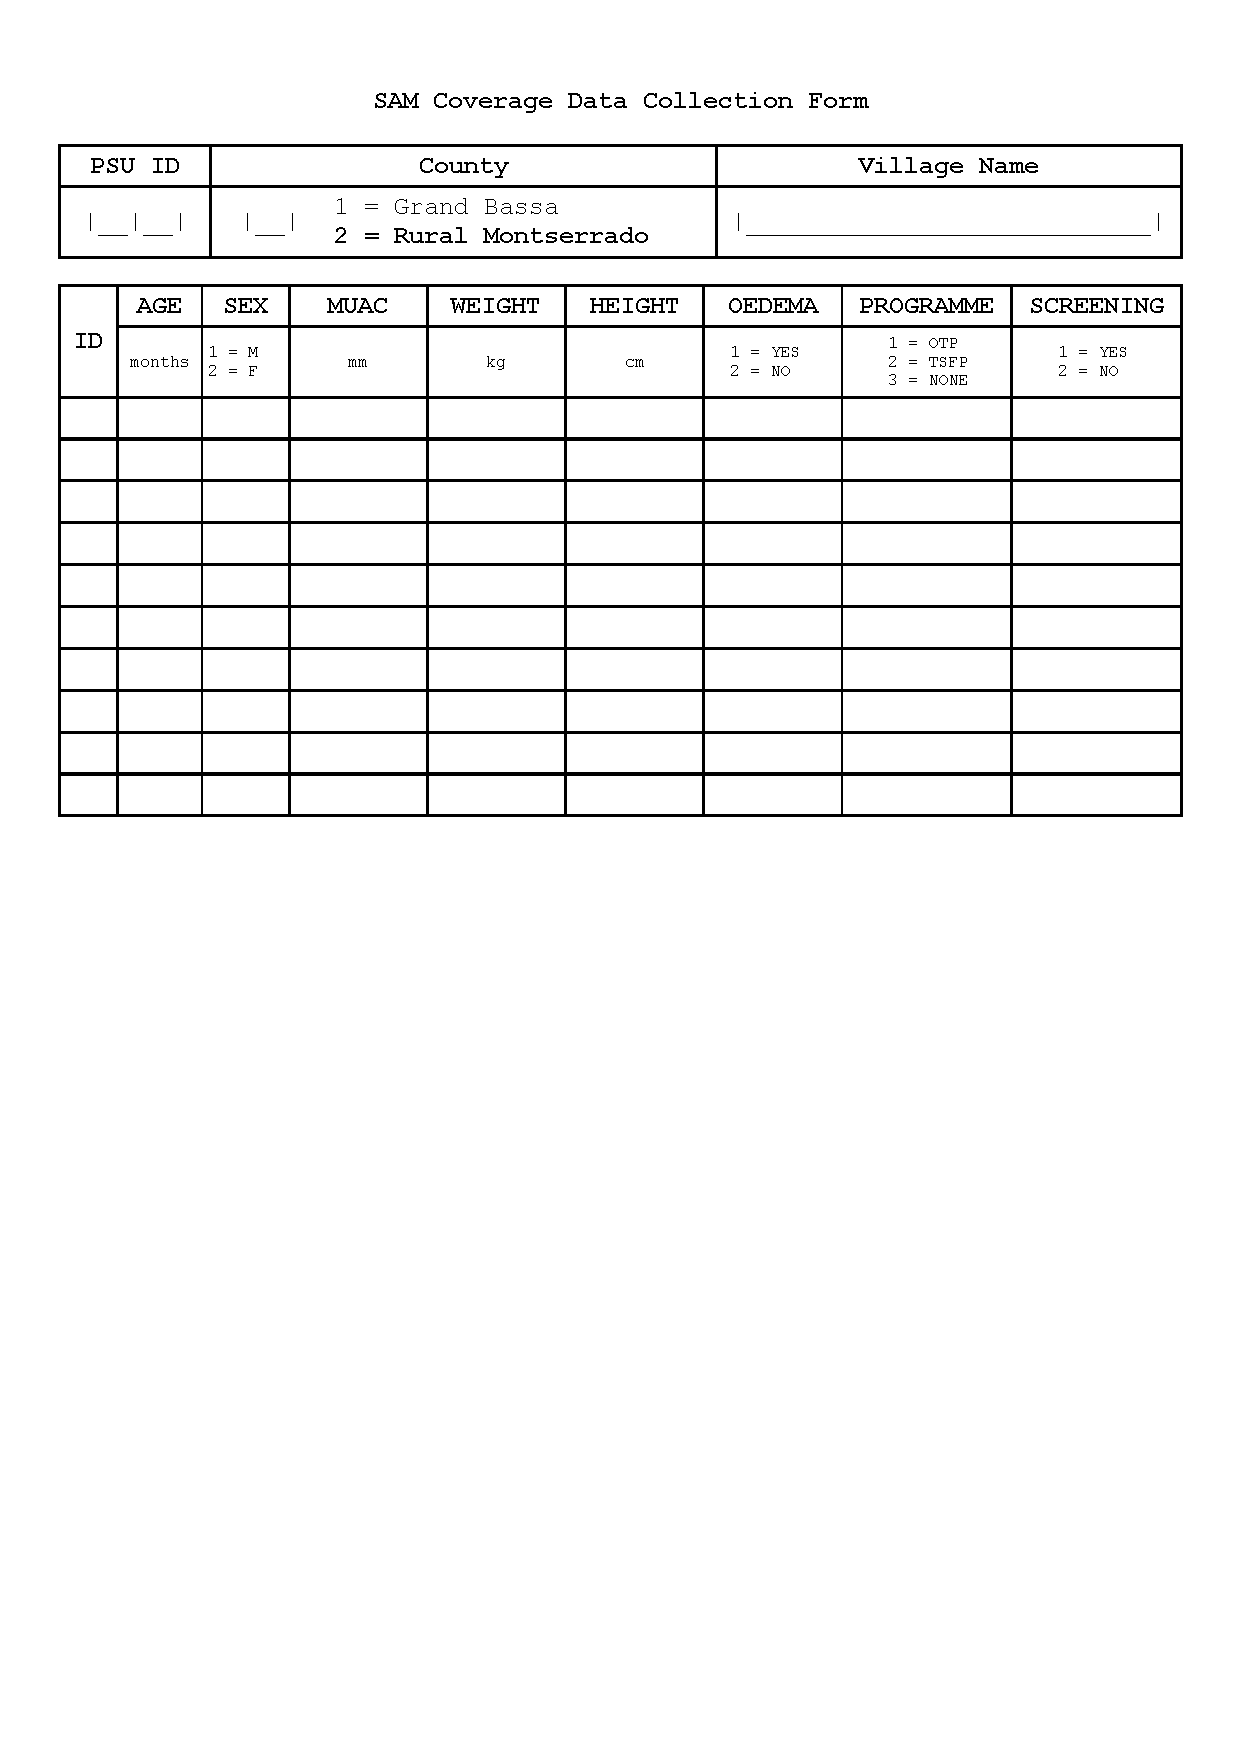
\includegraphics[width=0.9\linewidth]{forms/samForm} 

}

\caption{SAM coverage survey sample/template form}\label{fig:samform}
\end{figure}

~

The data collected using the tabular forms allows for estimation of
coverage. They do not, however, allow one to know the reasons for
coverage failure. To collect this data we applied a ``barriers''
questionnaire to the mothers/carers of uncovered SAM cases. Here is an
example of a barriers questionnaire:

\newpage

\begin{figure}[H]

{\centering 
\includegraphics[width=0.9\linewidth]{forms/samBarriersForm} 

}

\caption{SAM coverage barriers survey sample/template form}\label{fig:sambarriers}
\end{figure}

\newpage

\hypertarget{survey-for-children-6-59-months-and-their-mothers}{%
\subsubsection{Survey for children 6-59 months and their
mothers}\label{survey-for-children-6-59-months-and-their-mothers}}

For the survey for children 6-59 months, following is a sample/template
questionnaire used.

\begin{figure}[H]

{\centering 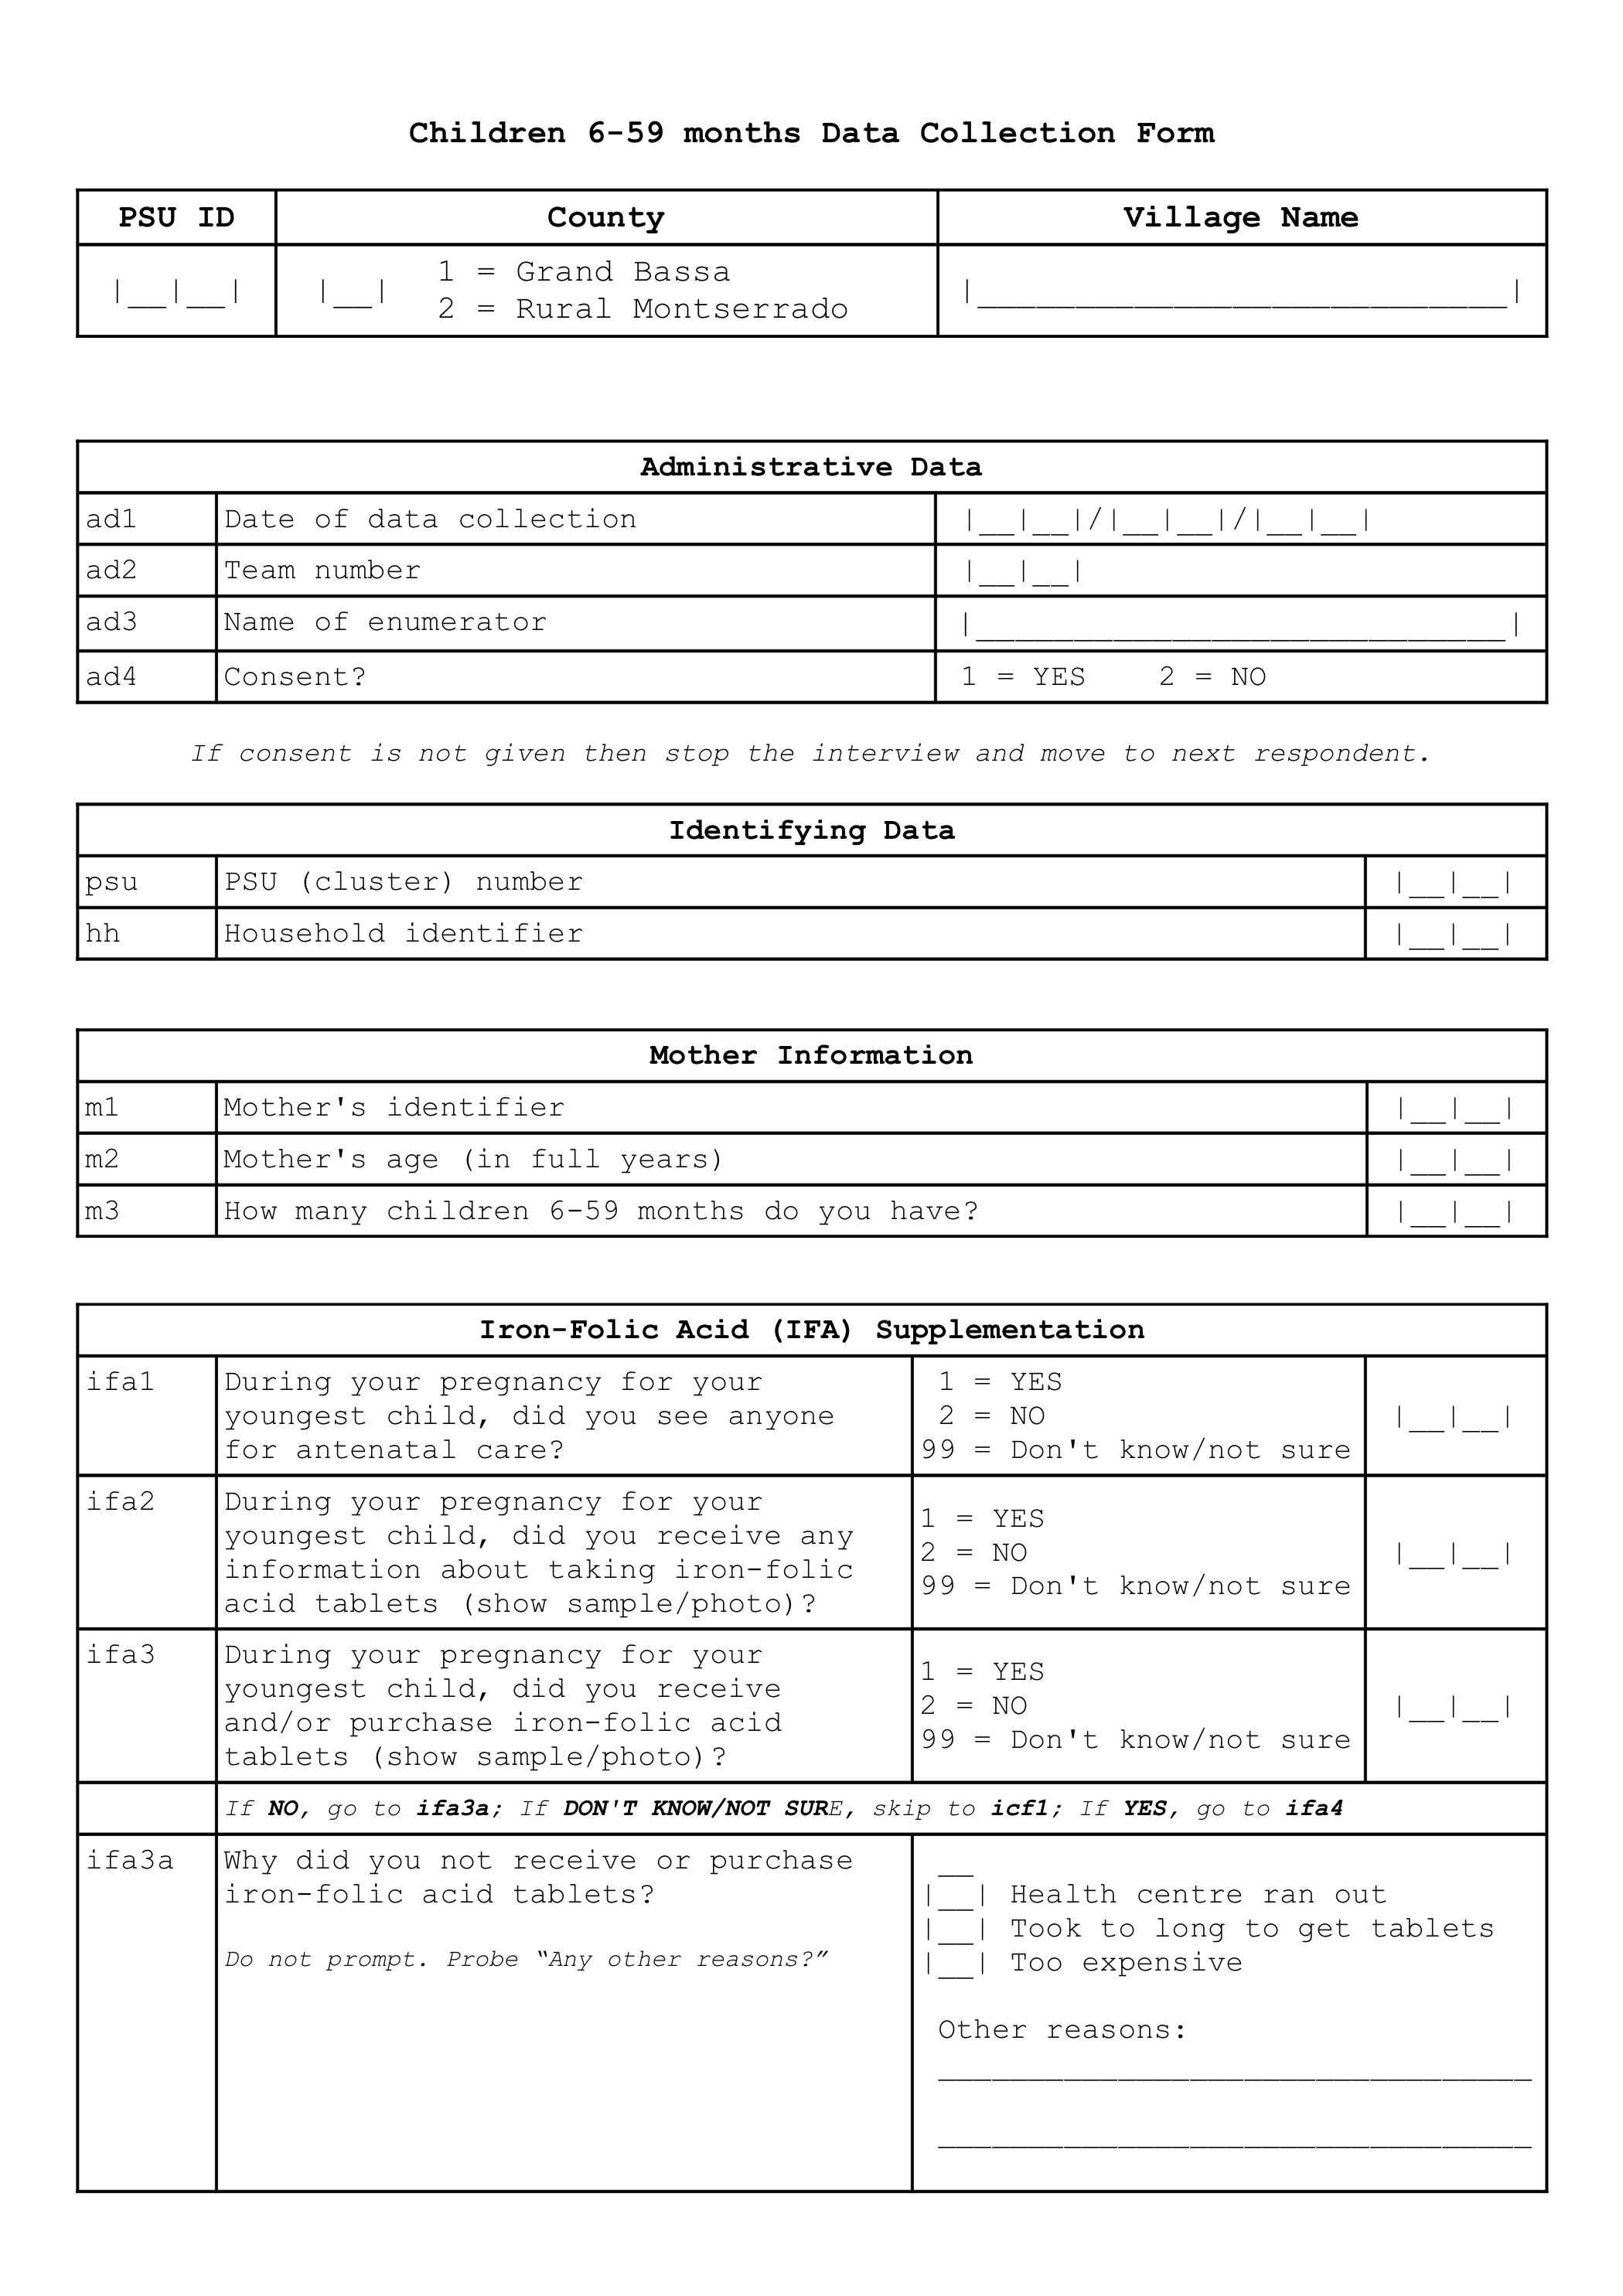
\includegraphics[width=0.9\linewidth]{forms/childForm1} 

}

\caption{Children 6-59 months old and their mothers survey sample/template form}\label{fig:childform1}
\end{figure}\begin{figure}[H]

{\centering 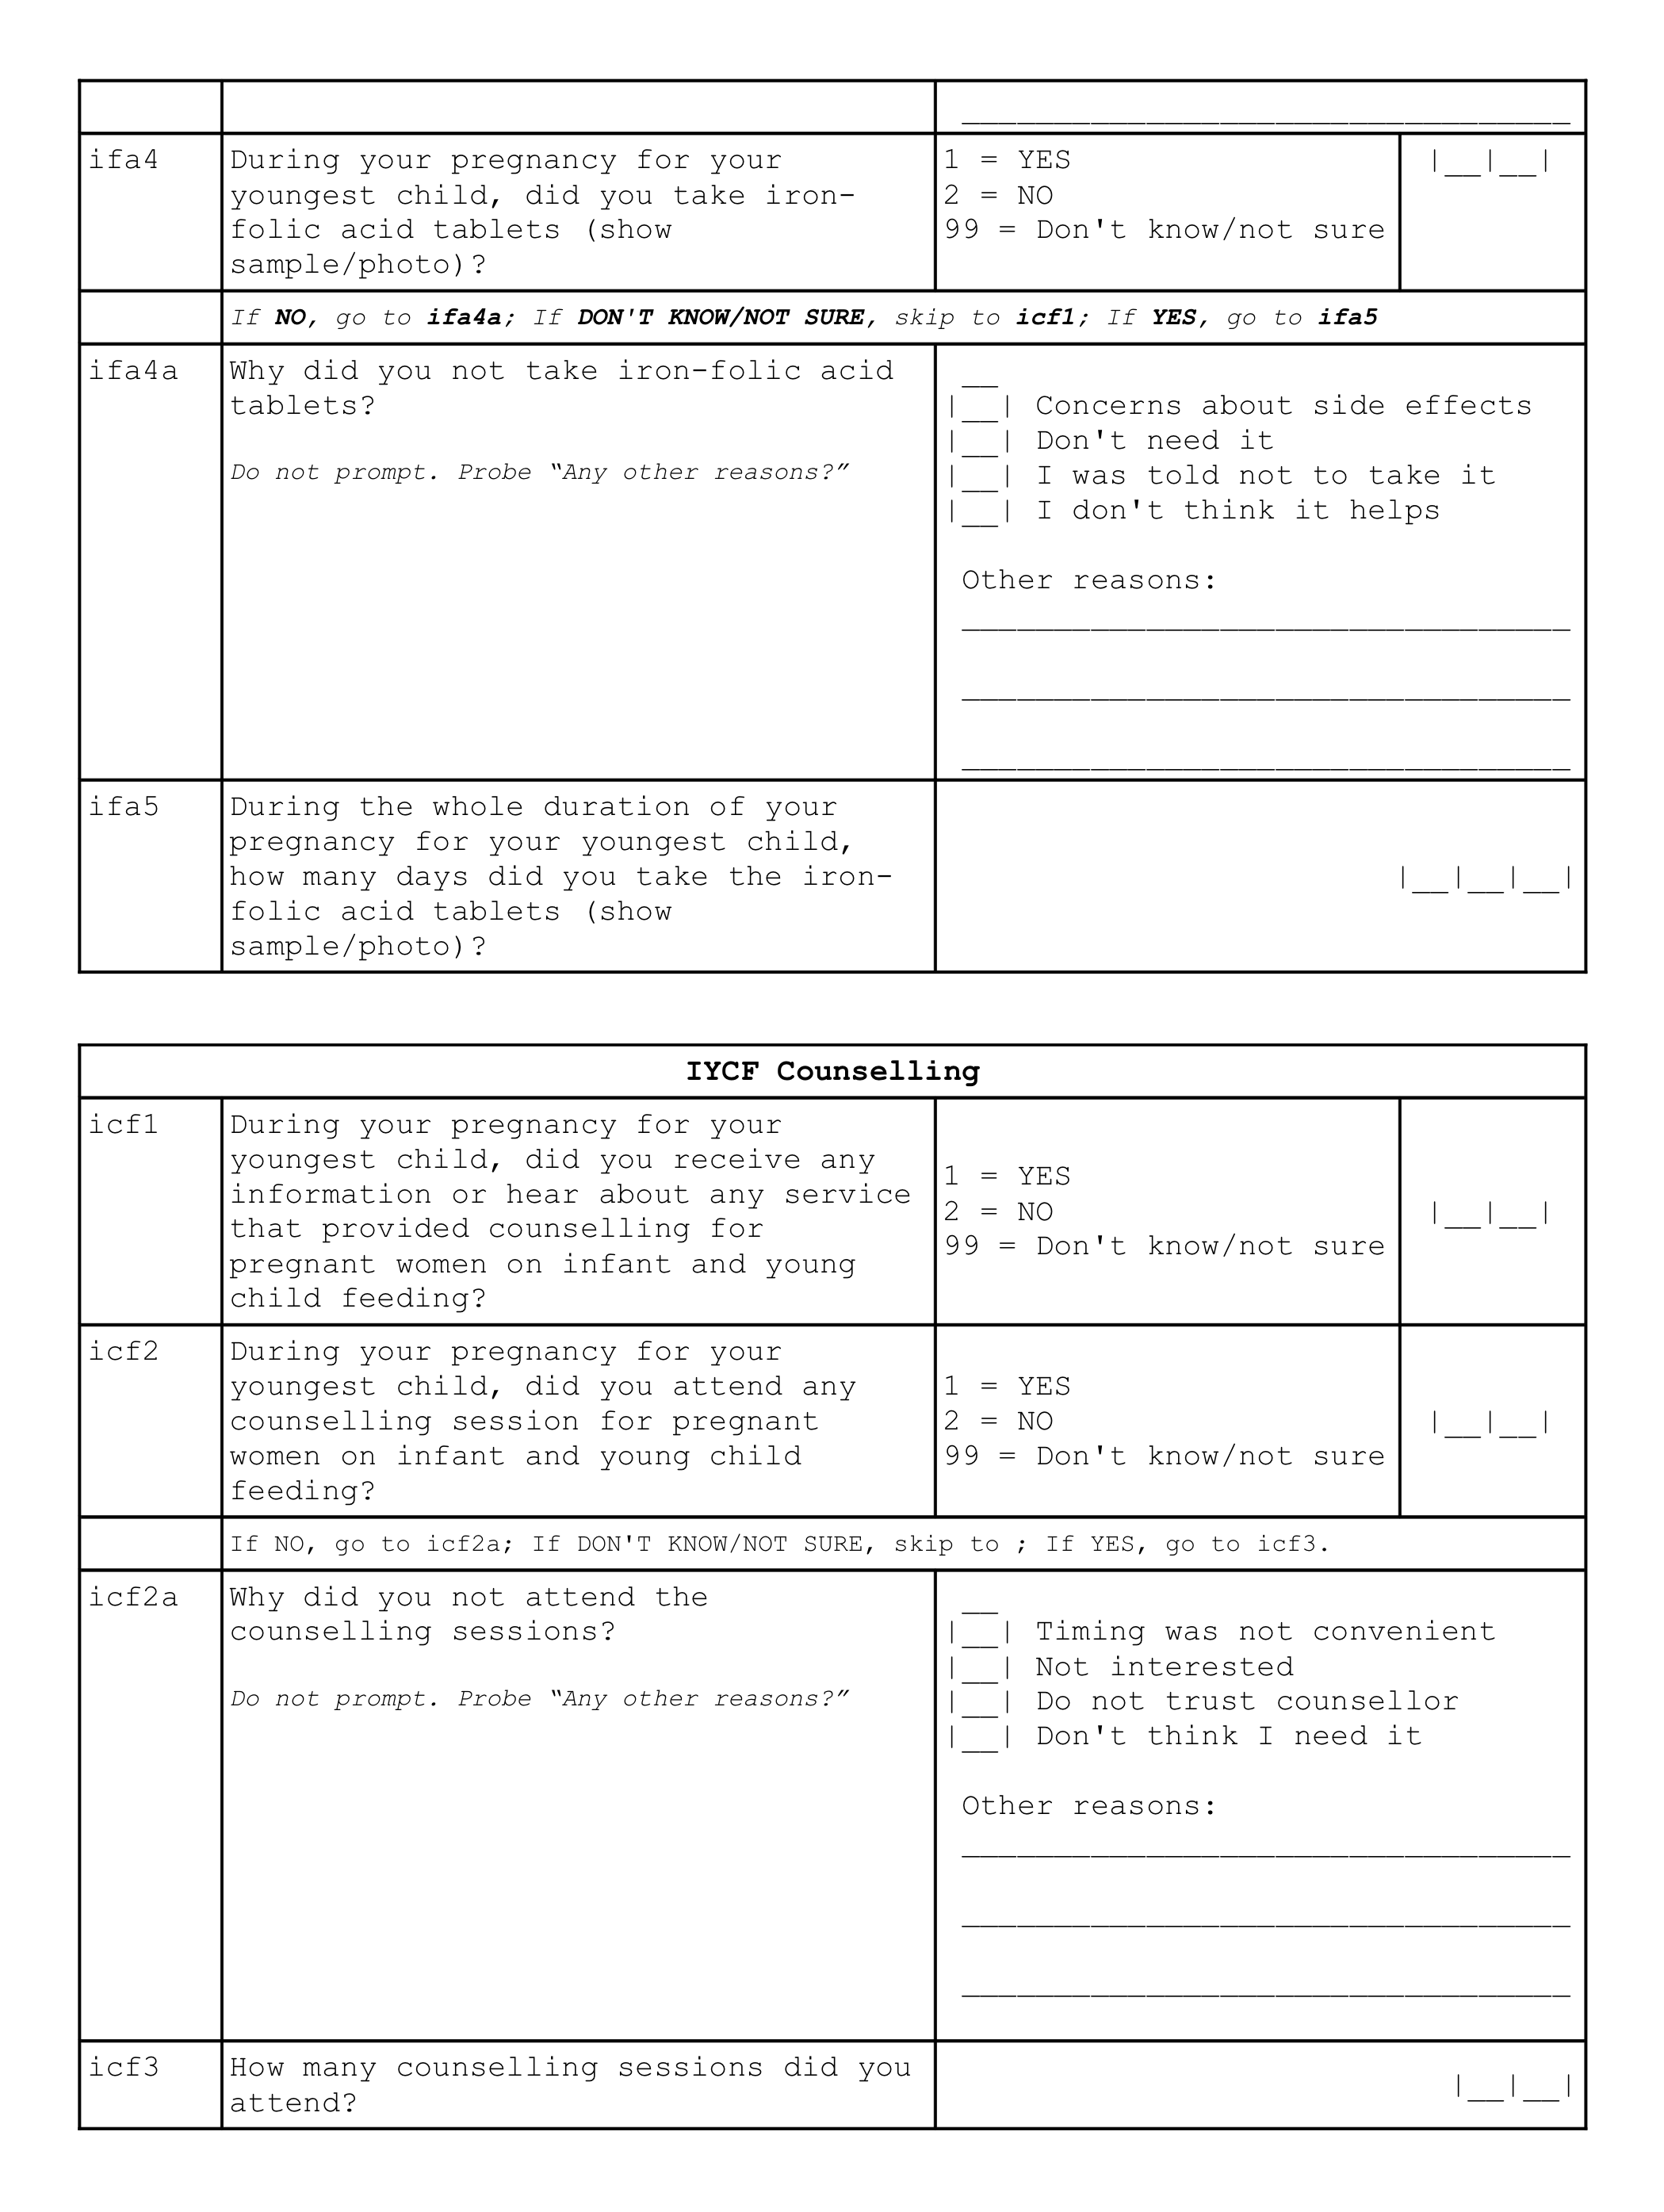
\includegraphics[width=0.9\linewidth]{forms/childForm2} 

}

\caption{Children 6-59 months old and their mothers survey sample/template form}\label{fig:childform1}
\end{figure}\begin{figure}[H]

{\centering 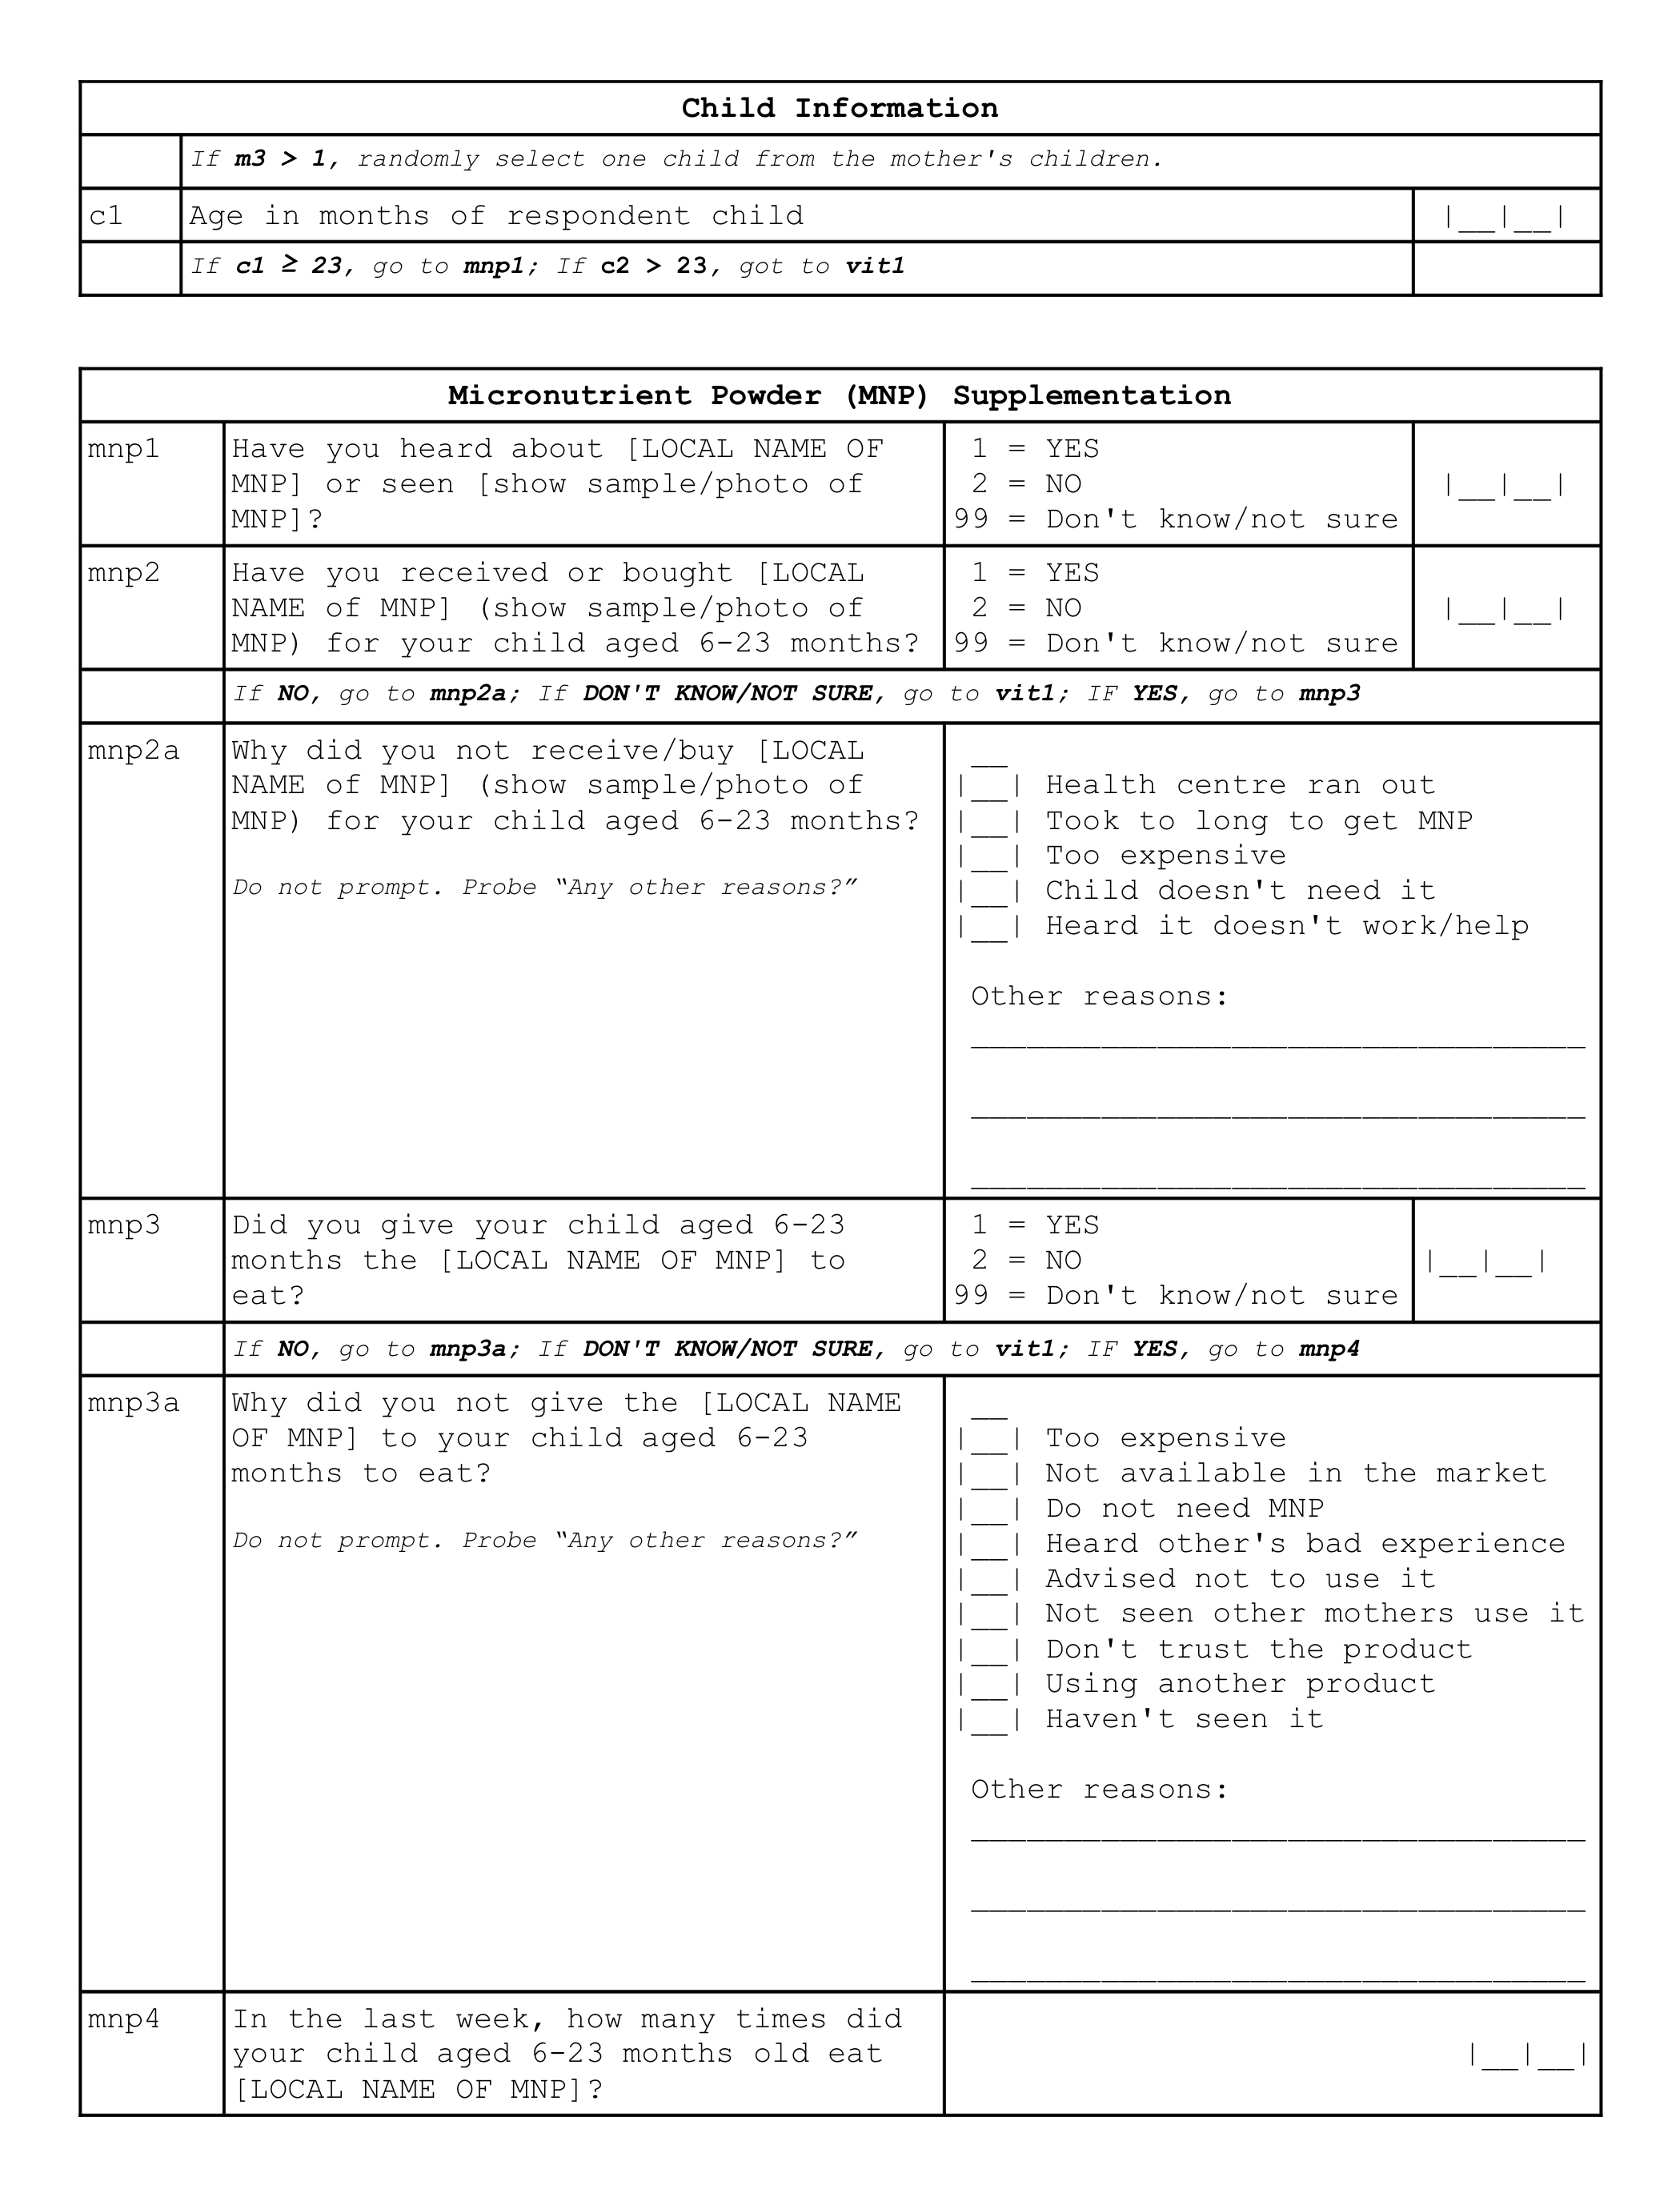
\includegraphics[width=0.9\linewidth]{forms/childForm3} 

}

\caption{Children 6-59 months old and their mothers survey sample/template form}\label{fig:childform1}
\end{figure}\begin{figure}[H]

{\centering 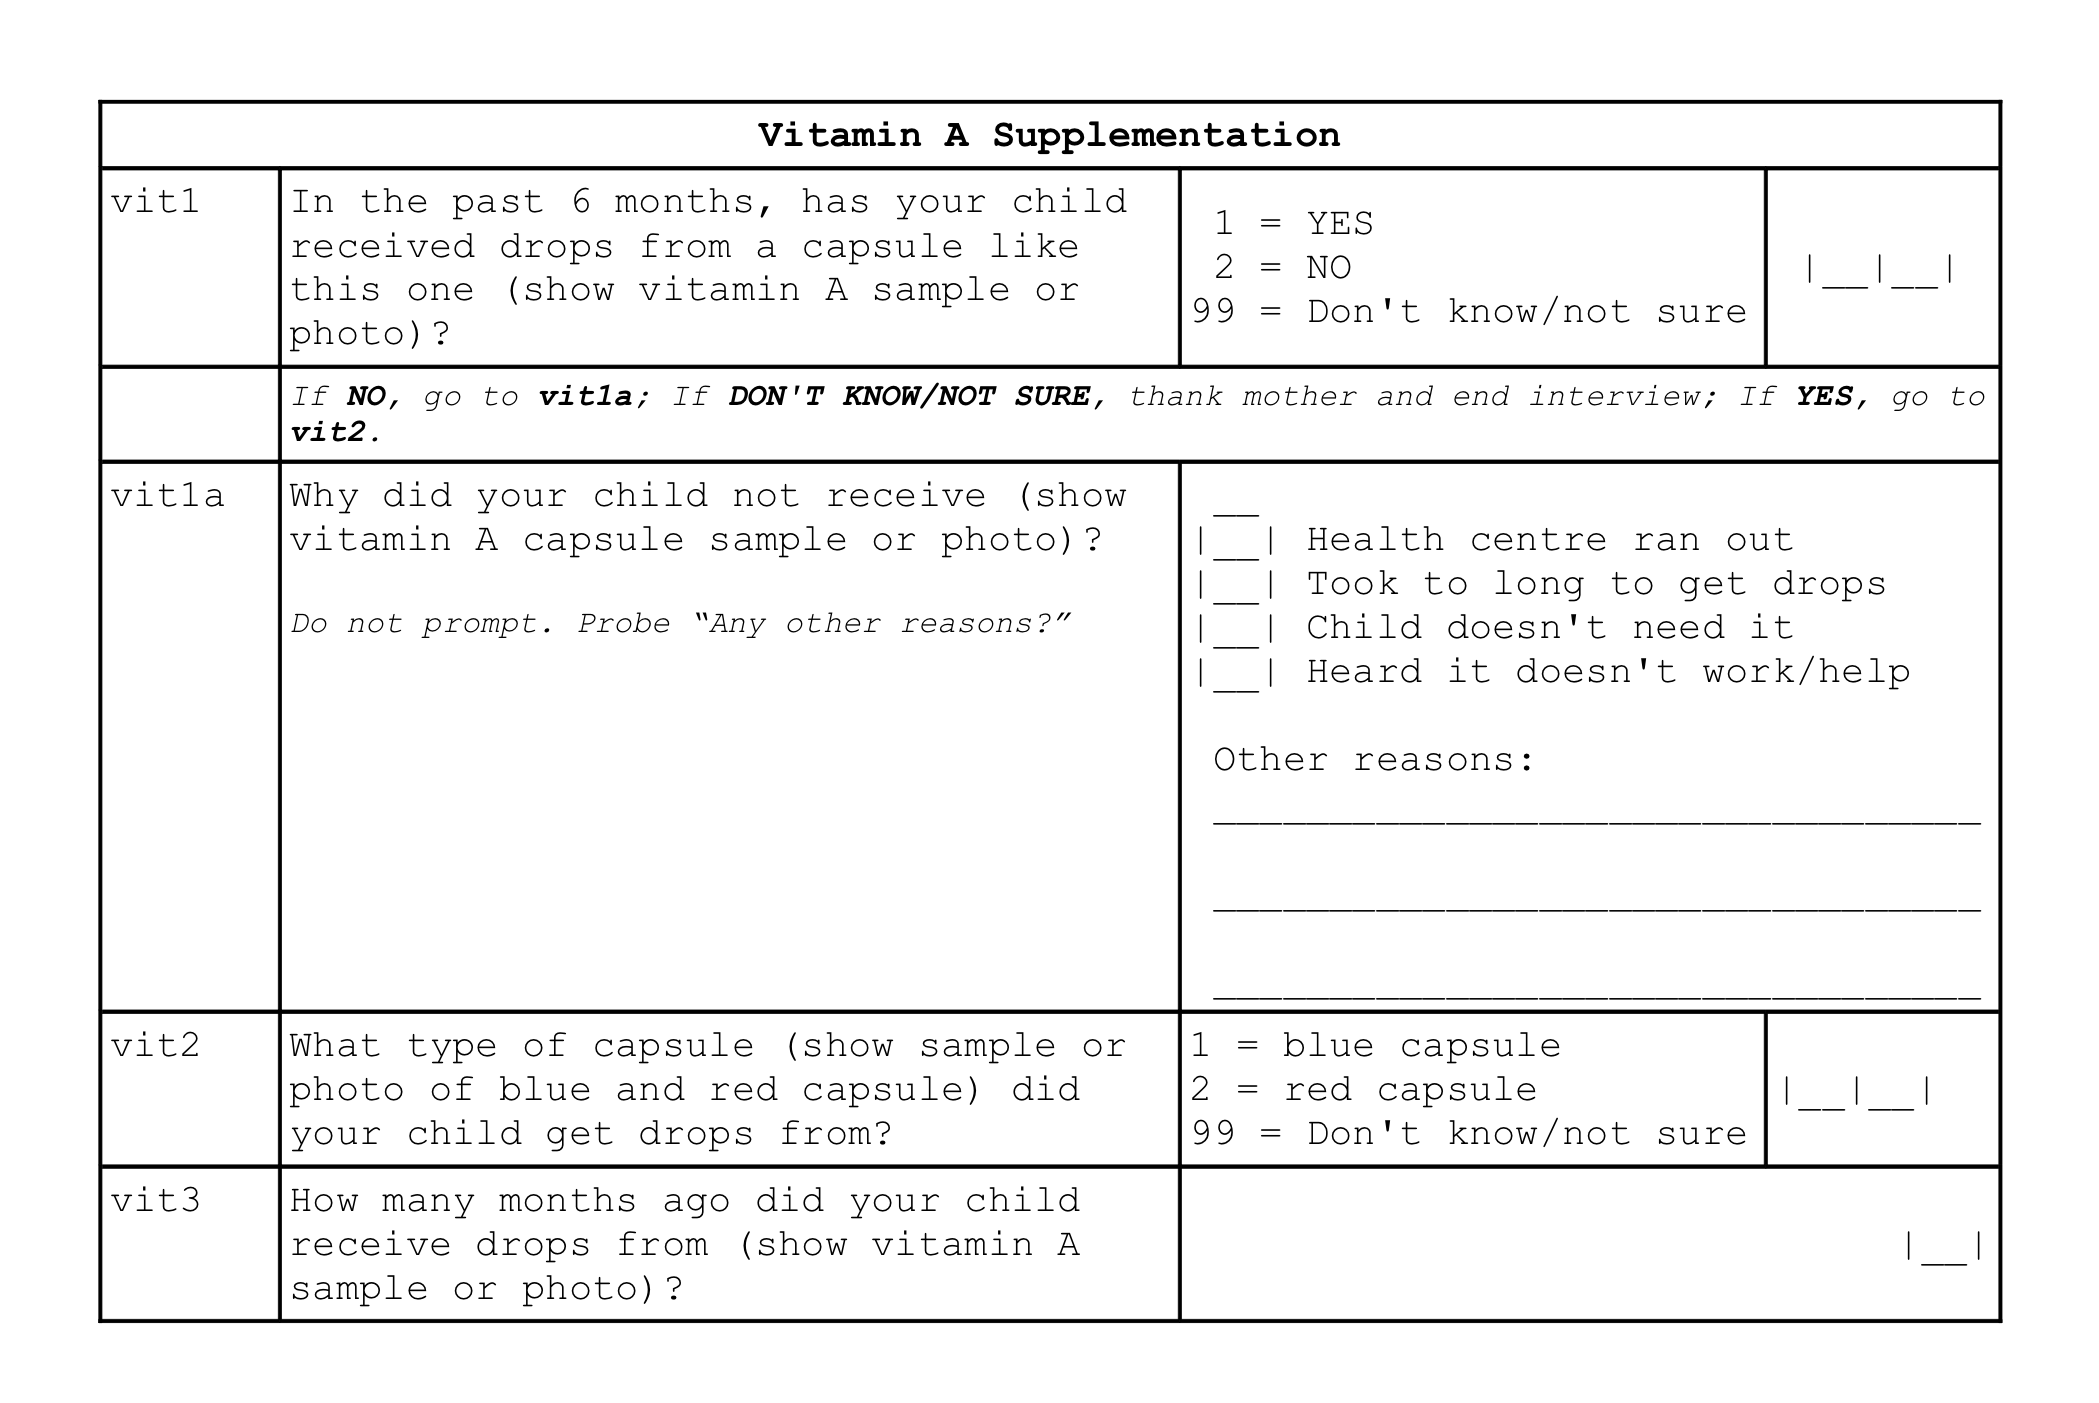
\includegraphics[width=0.9\linewidth]{forms/childForm4} 

}

\caption{Children 6-59 months old and their mothers survey sample/template form}\label{fig:childform1}
\end{figure}

\hypertarget{using-open-data-kit}{%
\subsubsection{Using Open Data Kit}\label{using-open-data-kit}}

Based on the template forms described above, a digital data collection
system using Open Data Kit (ODK) was developed. These forms are
available as a
\href{https://github.com/validmeasures/liberiaS3Mforms}{Github
repository}. The system is composed of two forms.

\hypertarget{village-form}{%
\paragraph{Village form}\label{village-form}}

This form (\texttt{liberiaCoverageVillageForm.xlsx} and
\texttt{liberiaCoverageVillageForm.xml}) collected information on the
villages or primary sampling units (PSU) selected for the Liberia
Coverage Survey. This information includes:

\begin{enumerate}
\def\labelenumi{\arabic{enumi}.}
\item
  County name (and identifier)
\item
  Village name (and identifier)
\item
  Village population size
\item
  Village geocoordinates
\end{enumerate}

\hypertarget{coverage-form}{%
\paragraph{Coverage form}\label{coverage-form}}

This form (\texttt{liberiaCoverage.xlsx} and
\texttt{liberiaCoverage.xml}) collected information on the various
coverage indicators assessed in the Liberia Coverage Survey:

\begin{enumerate}
\def\labelenumi{\arabic{enumi}.}
\item
  CMAM coverage
\item
  Iron-folic acid supplementation coverage
\item
  IYCF counselling coverage
\item
  Micronutrient powder supplementation coverage
\item
  Vitamin A supplementation coverage
\end{enumerate}

The coverage form was developed in such a way that it implements the
survey as per survey design such that the modules for IFA coverage, IYCF
counselling coverage, MNP supplementation coverage and vitamin A
supplementation coverage are only shown based on the sampling interval
for a particular primary sampling unit (PSU) and based on the different
eligibility requirements for each coverage survey module.

\hypertarget{data-analyses}{%
\subsection{Data analyses}\label{data-analyses}}

Data analysis was performed using R language for statistical computing
\citep{R:2018}.

\hypertarget{analytical-approach-for-estimating-coverage-indicators}{%
\subsubsection{Analytical approach for estimating coverage
indicators}\label{analytical-approach-for-estimating-coverage-indicators}}

Data analysis procedures accounted for the sample design.

\begin{itemize}
\item
  This survey is a two-stage sample. Subjects are sampled from a small
  number of primary sampling units (PSUs).
\item
  This survey is \textbf{not} prior weighted. This means that per-PSU
  sampling weights will be needed. These are usually the populations of
  the PSU.
\end{itemize}

For this survey, the \emph{blocked weighted bootstrap} estimation
approach was used:

\begin{itemize}
\item
  \textbf{Blocked} : The block corresponds to the PSU or cluster.
\item
  \textbf{Weighted} : The sampling procedure for this survey does not
  use population proportional sampling to weight the sample prior to
  data collection as is done with SMART type surveys. This means that a
  posterior weighting procedure is required. The ``roulette wheel''
  algorithm to weight (i.e.~by population) the selection probability of
  PSUs in bootstrap replicates will be utilised.
\end{itemize}

A total of \texttt{m} PSUs are sampled \emph{with-replacement} from the
survey dataset where \texttt{m} is the number of PSUs in the survey
sample. Individual records within each PSU are then sampled
\emph{with-replacement}. A total of n' records are sampled
\emph{with-replacement} from each of the selected PSUs where \texttt{n}
is the number of individual records in a selected PSU. The resulting
collection of records replicates the original survey in terms of both
sample design and sample size. A large number of replicate surveys are
taken (minimum of \(r = 399\) replicate surveys but this can be
changed). The required statistic (e.g.~the mean of an indicator value)
is applied to each replicate survey. The reported estimate consists of
the 50th (point estimate), 2.5th (lower 95\% confidence limit), and the
97.5th (upper 95\% confidence limit) percentiles of the distribution of
the statistic observed across all replicate surveys. The blocked
weighted bootstrap procedure is outlined in Figure
\ref{fig:indicators31}.

The principal advantages of using a bootstrap estimator are:

\begin{itemize}
\item
  Bootstrap estimators work well with small sample sizes.
\item
  The method is \emph{non-parametric} and uses empirical rather than
  theoretical distributions. There are no assumptions of things like
  normality to worry about.
\item
  The method allows estimation of the sampling distribution of almost
  any statistic using only simple computational methods.
\end{itemize}

\newpage

\begin{figure}[H]

{\centering 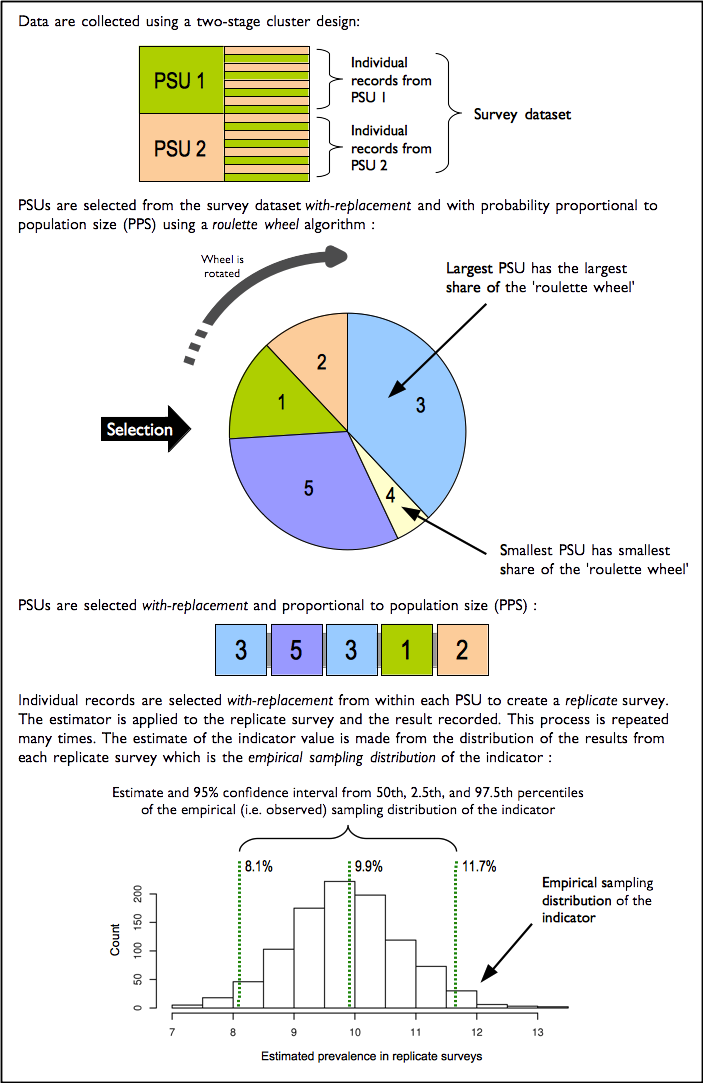
\includegraphics[width=9.76in]{figures/bbw} 

}

\caption{The blocked weighted bootstrap}\label{fig:indicators31}
\end{figure}

\hypertarget{analytical-approach-for-mapping-coverage-indicators}{%
\subsubsection{Analytical approach for mapping coverage
indicators}\label{analytical-approach-for-mapping-coverage-indicators}}

The indicator mapping will create a surface map of indicator values
using spatial interpolation. There are various approaches and methods of
spatial interpolation, the main differences are determined by the
weights applied to the point dataset to estimate values at each of the
unknown points of the surface map. For the Liberia coverage survey,
spatial interpolation will be performed using the inverse distance
weighting (IDW) method. As the name implies, the IDW method uses weights
that are inversely proportional to the distance of a point being
estimated from the sampling point locations
\citep{isaaks1989applied, diggle2007mbg, diggle2013statistical}. This
can be mathematically demonstrated as follows:

~

\[\begin{aligned}
\hat{v} & ~ = ~ \frac{\displaystyle \sum\limits_{i = 1}^{n} \frac{1}{d_{i}^{p}}v_{i}}{\displaystyle \sum\limits_{i = 1}^{n}\frac{1}{d_{i}^{p}}} \\
\\
where: & \\
\\
d_1 \ldots d_n & ~ = ~ \text{distances from each } n \text{ sampling points to estimation point} \\
p & ~ = ~ \text{power of the distance} \\
v_1 \ldots v_n & ~ = ~ \text{sample values}
\end{aligned}\]

~

The power of the distance \texttt{p} is an important aspect of the IDW
method for point estimation. The influence of \texttt{p} to the weights
applied to the point estimation is such that as \texttt{p} approaches 0,
the weights become more similar, thereby giving more weight to the
nearest sample values. As \texttt{p} approaches \(\infty\), the weights
become more different from each other, thereby giving more weight to the
closest sample. The power of the distance \texttt{p} has been
traditionally set at 2 for convenience and ease of calculations. In
theory, given a set \texttt{p}, IDW calculations can be performed using
manual calculations aided by a spreadsheet and / or a calculator as it
requires fewer calculations. For the Liberia Coverage Survey, \texttt{p}
will be initially set at 2 and then cross-validation (see below) will be
applied to optimise \texttt{p} to a value that minimises the estimation
errors at each of the sampling point locations.

Cross-validation is a technique applied to validate predictive models.
It assesses how accurately the predictive model performs in practice.
IDW is one of the simplest model-based interpolation methods available,
but ideally would still require a form of cross-validation to determine
the optimal value of the distance power \texttt{p} (described above).

A two-fold cross validation \citep{bivand2008applied} in which data
points are randomly split into two sets of equal size, with one set
assigned as the validation data for testing the model, and the other set
as the training data. The validation data is then interpolated using the
IDW method with an initial \texttt{p} of 2 and the resulting predictions
were compared with the training data. Comparison is made using the sum
of the squared residuals between the predicted values and the observed
values to report errors. Optimisation is then performed by replicating
the two-fold cross validation process 100 times using randomly generated
values for \texttt{p}. Out of these replicates, the value of \texttt{p}
that provided prediction results with the minimum errors is selected as
the distance power for the eventual interpolation performed.

\hypertarget{results-and-discussion}{%
\section{Results and Discussion}\label{results-and-discussion}}

\hypertarget{iron-folic-acid-supplementation-coverage}{%
\subsection{Iron-Folic Acid Supplementation
Coverage}\label{iron-folic-acid-supplementation-coverage}}

Figure \ref{fig:ifa1} and Table \ref{tab:ifa2} presents a summary of the
IFA supplementation coverage indicators.

\begin{figure}[H]

{\centering 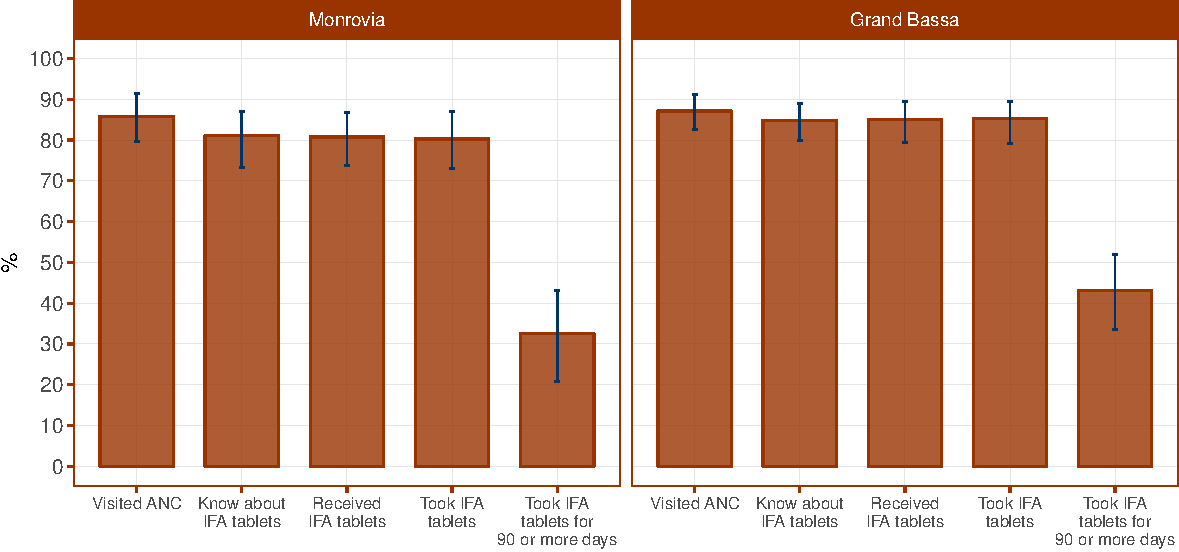
\includegraphics{liberiaCoverageReport_files/figure-latex/ifa1-1} 

}

\caption{Iron-Folic Acid Supplementation Coverage}\label{fig:ifa1}
\end{figure}

\rowcolors{2}{gray!6}{white}\begin{table}[H]

\caption{\label{tab:ifa2}Iron-Folic Acid Supplementation Coverage}
\centering
\resizebox{\linewidth}{!}{
\fontsize{10}{12}\selectfont
\begin{tabular}[t]{lrrrrrr}
\hiderowcolors
\toprule
\multicolumn{1}{c}{\bfseries  } & \multicolumn{3}{c}{\bfseries Monrovia} & \multicolumn{3}{c}{\bfseries Grand Bassa} \\
\cmidrule(l{2pt}r{2pt}){2-4} \cmidrule(l{2pt}r{2pt}){5-7}
\multicolumn{1}{c}{\textbf{Indicator}} & \multicolumn{1}{c}{\textbf{Estimate}} & \multicolumn{1}{c}{\textbf{95\% LCL}} & \multicolumn{1}{c}{\textbf{95\% UCL}} & \multicolumn{1}{c}{\textbf{Estimate}} & \multicolumn{1}{c}{\textbf{95\% LCL}} & \multicolumn{1}{c}{\textbf{95\% UCL}}\\
\midrule
\showrowcolors
Visited ANC & 85.80 & 79.70 & 91.39 & 87.15 & 82.67 & 91.16\\
Know about IFA tablets & 81.11 & 73.24 & 86.96 & 84.87 & 79.98 & 88.96\\
Received IFA tablets & 80.75 & 73.69 & 86.84 & 85.01 & 79.41 & 89.40\\
Took IFA tablets & 80.28 & 73.12 & 87.07 & 85.23 & 79.10 & 89.51\\
Took IFA tablets for 90 or more days & 32.56 & 20.82 & 43.04 & 43.17 & 33.64 & 51.98\\
\bottomrule
\end{tabular}}
\end{table}\rowcolors{2}{white}{white}

The majority of mothers from the sample for Monrovia and Grand Bassa
have attended ANC during their last pregnancy, are aware of IFA tablets,
have received IFA tablets and have consumed IFA tablets.

Of the few who have not received IFA tablets despite attending ANC
during their last pregnancy, the main reasons for not getting IFA
tablets are shown in \ref{fig:ifa3a}

\begin{figure}[H]

{\centering 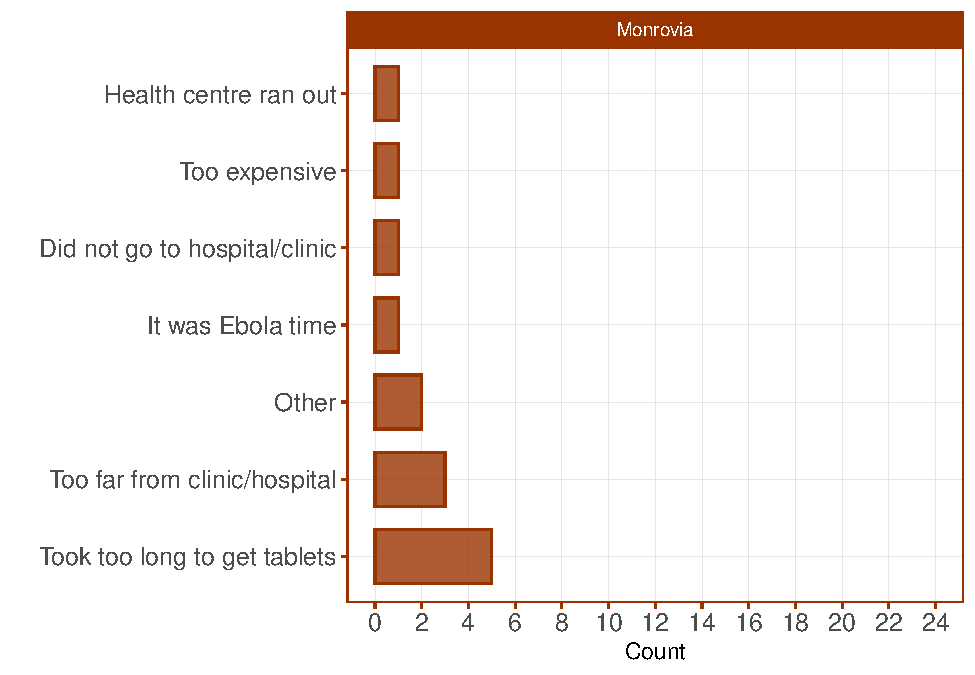
\includegraphics[width=8cm,height=6cm]{liberiaCoverageReport_files/figure-latex/ifa3a-1} 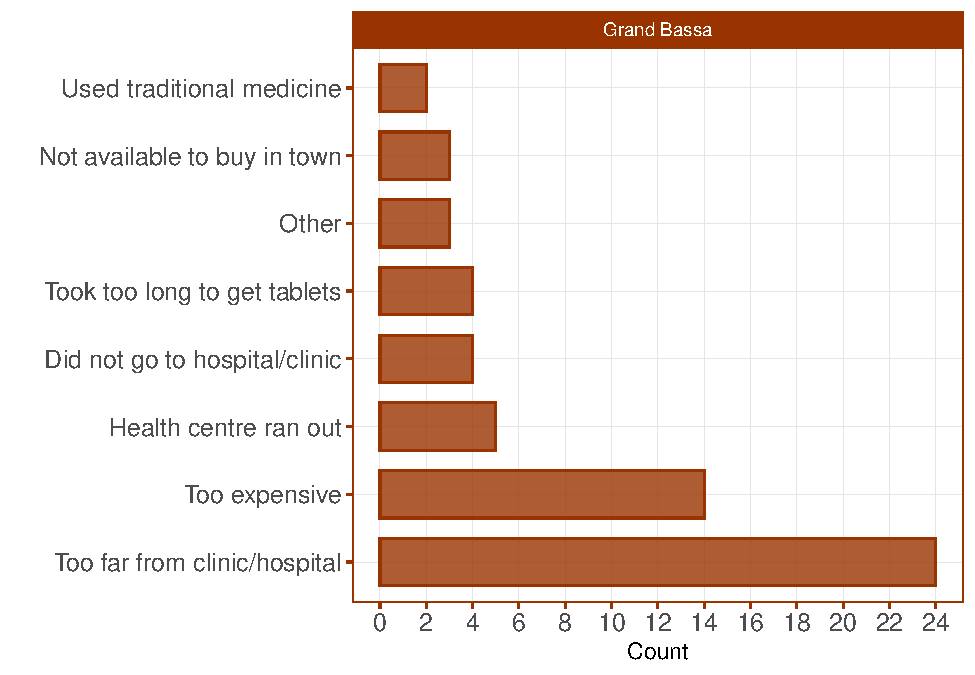
\includegraphics[width=8cm,height=6cm]{liberiaCoverageReport_files/figure-latex/ifa3a-2} 

}

\caption{Reasons for not receiving/purchasing iron-folic acid tablets}\label{fig:ifa3a}
\end{figure}

However, coverage of IFA falters significantly when length of IFA tablet
consumption is assessed. Only 33\% and 42\% of mothers in Monrovia and
Grand Bassa respectively have consumed IFA tablets for at least 90 days
during their last pregnancy.

On further analysis of the length of IFA tablet consumption, most
mothers in both Monrovia and Grand Bassa have consumed IFA tablets for
less than 60 months as shown in Figure @fig:ifa5). Median number of days
of IFA tablet consumption (shown by dotted lines in Figure
\ref{fig:ifa5}) is 56 and 52 days for Monrovia and Grand Bassa
respectively.

\begin{figure}[H]

{\centering 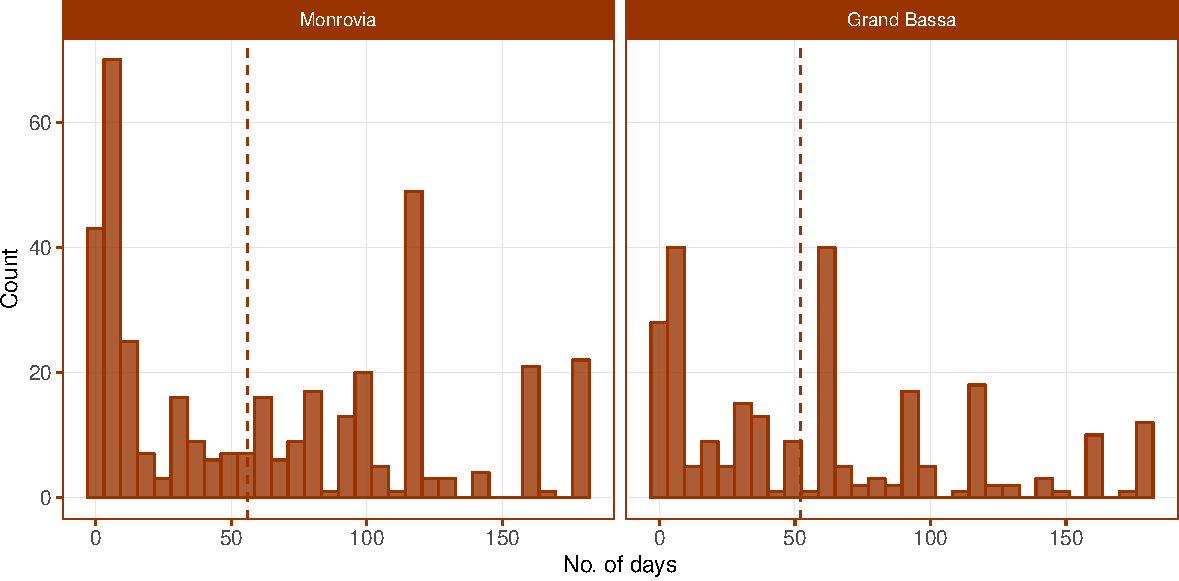
\includegraphics{liberiaCoverageReport_files/figure-latex/ifa5-1} 

}

\caption{Number of days mothers took IFA tablets during their last pregnancy}\label{fig:ifa5}
\end{figure}

The spatial distribution of IFA supplementation coverage is shown in
Figure \ref{fig:ifaMap1}. IFA supplementation coverage is lowest in the
eastern section of Monrovia and in the southern and eastern areas of
Grand Bassa.

\begin{figure}[H]

{\centering 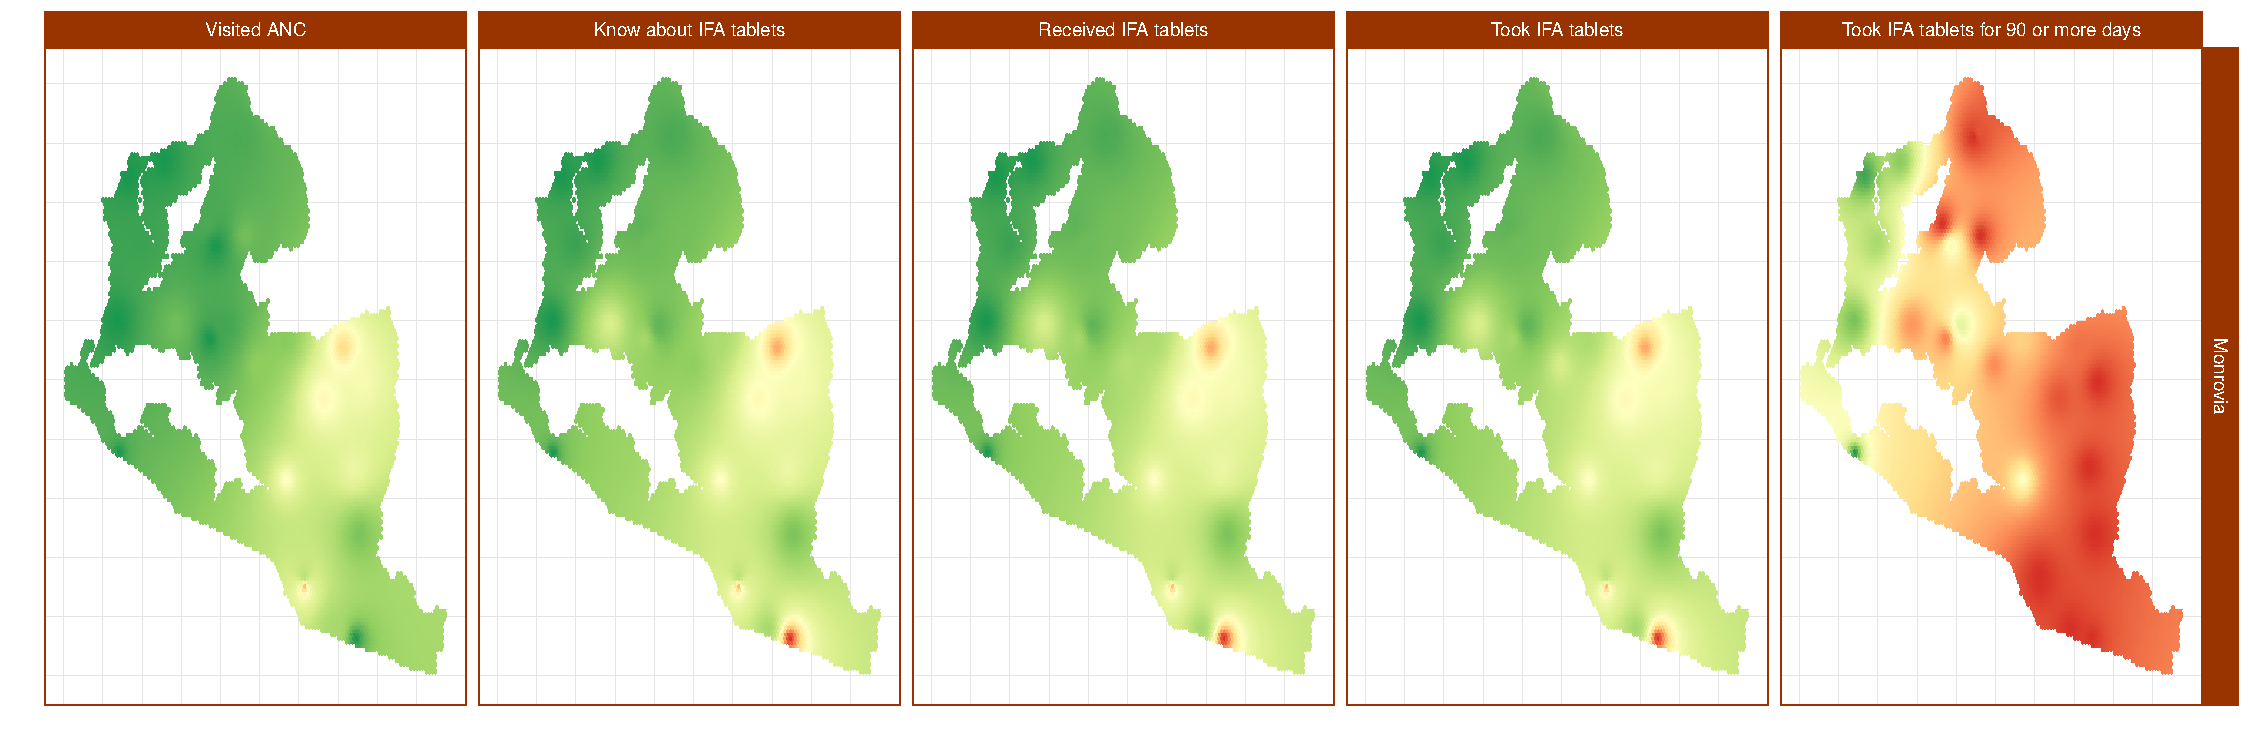
\includegraphics{liberiaCoverageReport_files/figure-latex/ifaMap1-1} 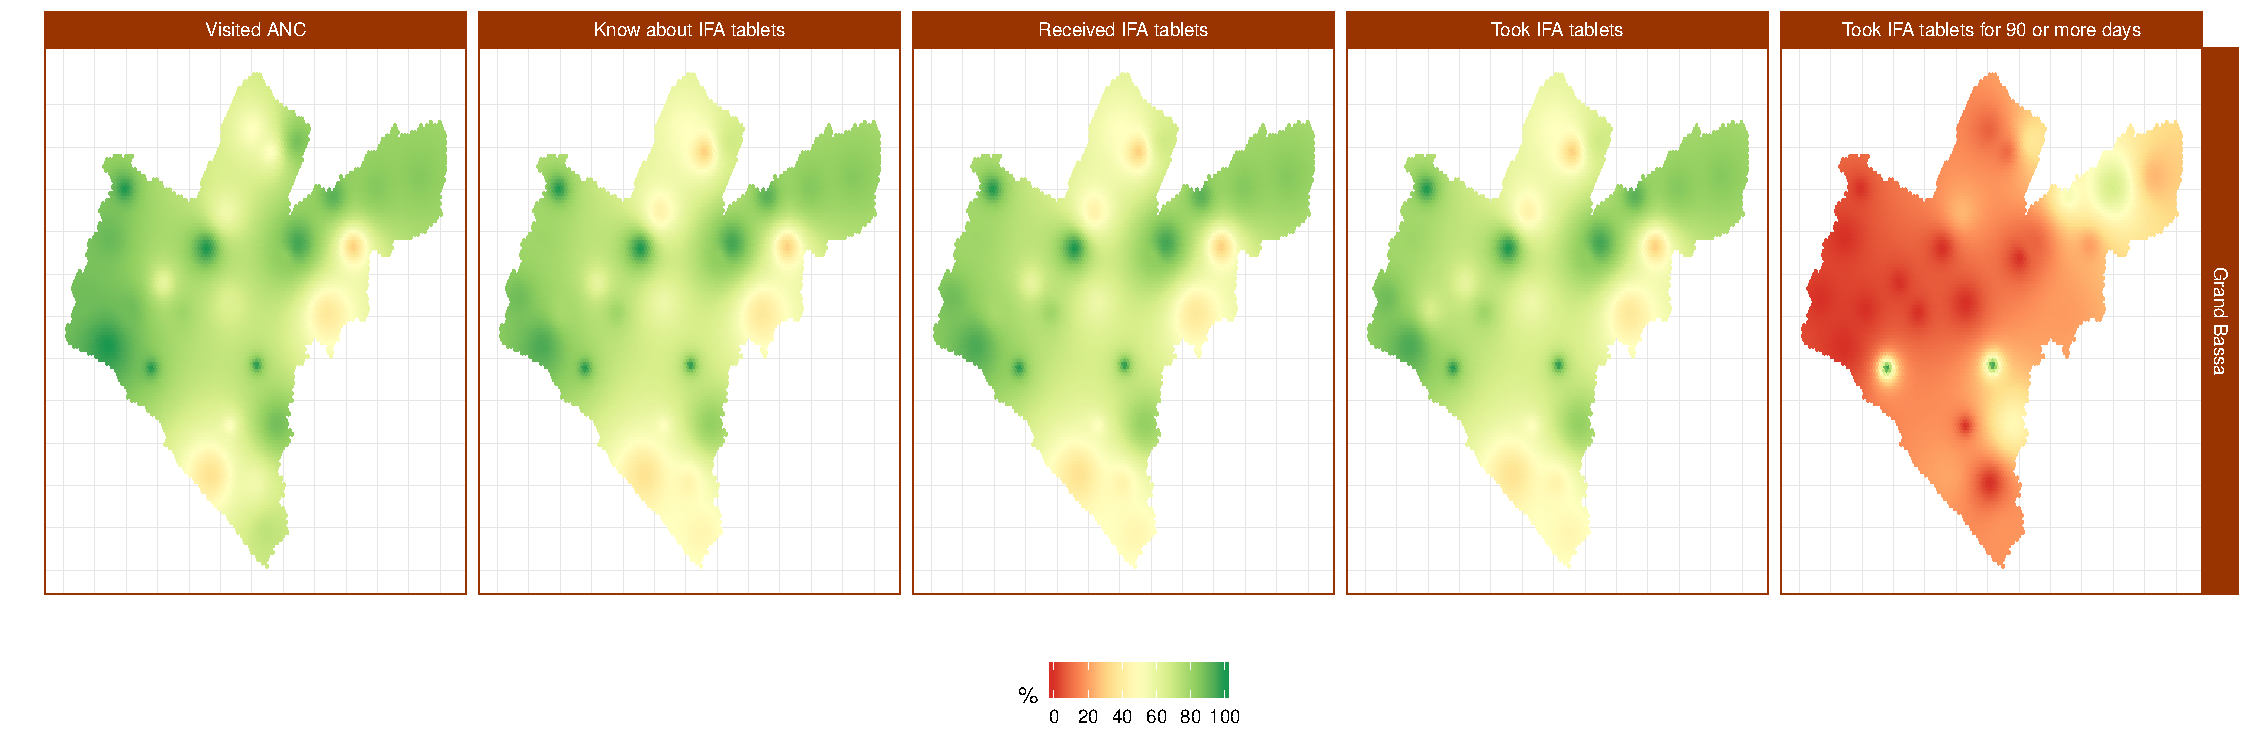
\includegraphics{liberiaCoverageReport_files/figure-latex/ifaMap1-2} 

}

\caption{Spatial Distribution of Iron Folic Acid Supplementation Coverage}\label{fig:ifaMap1}
\end{figure}

The spatial distribution of length (in days) of IFA tablet consumption
is shown in Figure \ref{fig:ifaMap2}. Areas with longest IFA tablet
consumption are at the northwest section of Monrovia and northeastern
areas of Grand Bassa.

\begin{figure}[H]

{\centering 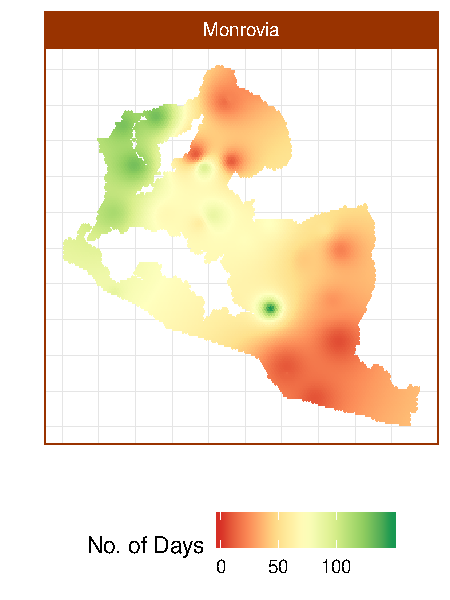
\includegraphics{liberiaCoverageReport_files/figure-latex/ifaMap2-1} 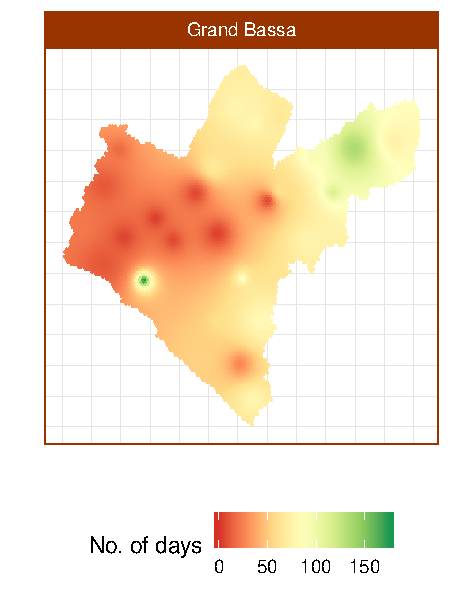
\includegraphics{liberiaCoverageReport_files/figure-latex/ifaMap2-2} 

}

\caption{Spatial Distribution of Number of Days IFA Consumption}\label{fig:ifaMap2}
\end{figure}

\newpage

\hypertarget{iycf-counselling-coverage}{%
\subsection{IYCF Counselling Coverage}\label{iycf-counselling-coverage}}

Knowledge of and attendance to IYCF counselling is both close to 80\%
for Monrovia and Grand Bassa (Figure \ref{fig:icf1} and Table
\ref{tab:icf2}).

\begin{figure}[H]

{\centering 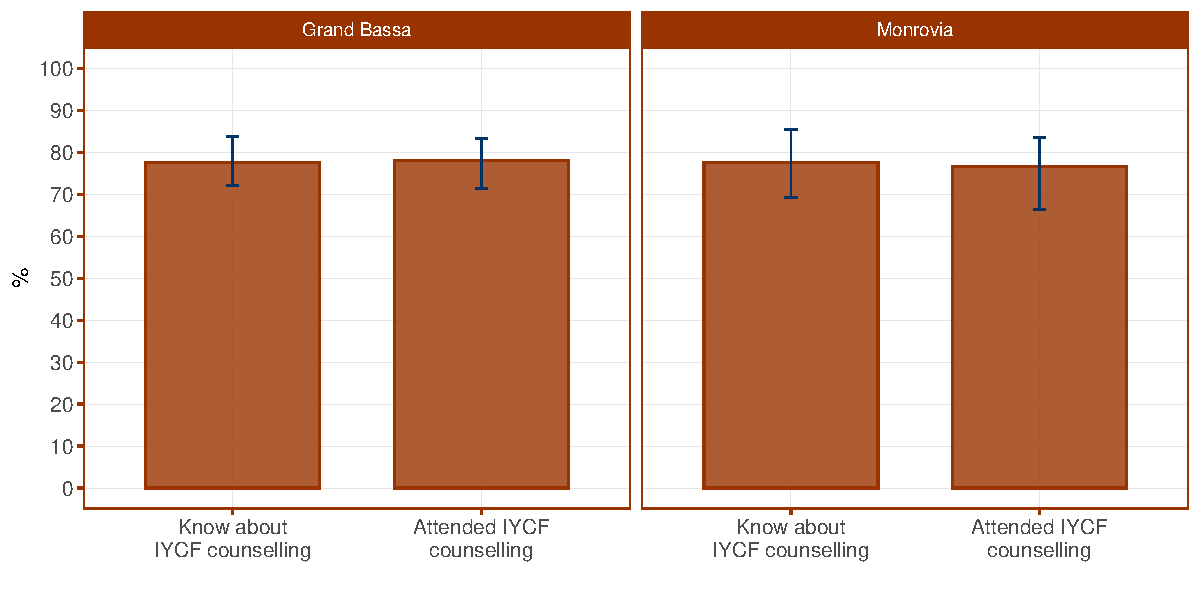
\includegraphics{liberiaCoverageReport_files/figure-latex/icf1-1} 

}

\caption{IYCF Counselling Coverage}\label{fig:icf1}
\end{figure}

\rowcolors{2}{gray!6}{white}\begin{table}[H]

\caption{\label{tab:icf2}IYCF Counselling Coverage}
\centering
\fontsize{10}{12}\selectfont
\begin{tabular}[t]{lrrrrrr}
\hiderowcolors
\toprule
\multicolumn{1}{c}{\bfseries  } & \multicolumn{3}{c}{\bfseries Monrovia} & \multicolumn{3}{c}{\bfseries Grand Bassa} \\
\cmidrule(l{2pt}r{2pt}){2-4} \cmidrule(l{2pt}r{2pt}){5-7}
\textbf{Indicator} & \textbf{Estimate} & \textbf{95\% LCL} & \textbf{95\% UCL} & \textbf{Estimate} & \textbf{95\% LCL} & \textbf{95\% UCL}\\
\midrule
\showrowcolors
Know about IYCF counselling & 77.62 & 69.24 & 85.42 & 77.47 & 72.09 & 83.75\\
Attended IYCF counselling & 76.55 & 66.31 & 83.43 & 78.12 & 71.27 & 83.27\\
\bottomrule
\end{tabular}
\end{table}\rowcolors{2}{white}{white}

Spatial distribution of IYCF counselling coverage is shown in Figure
\ref{fig:icfMap}. IYCF counselling coverage is at its lowest in sections
East of Monrovia and in the southern and eastern areas of Grand Bassa.

\begin{figure}[H]

{\centering 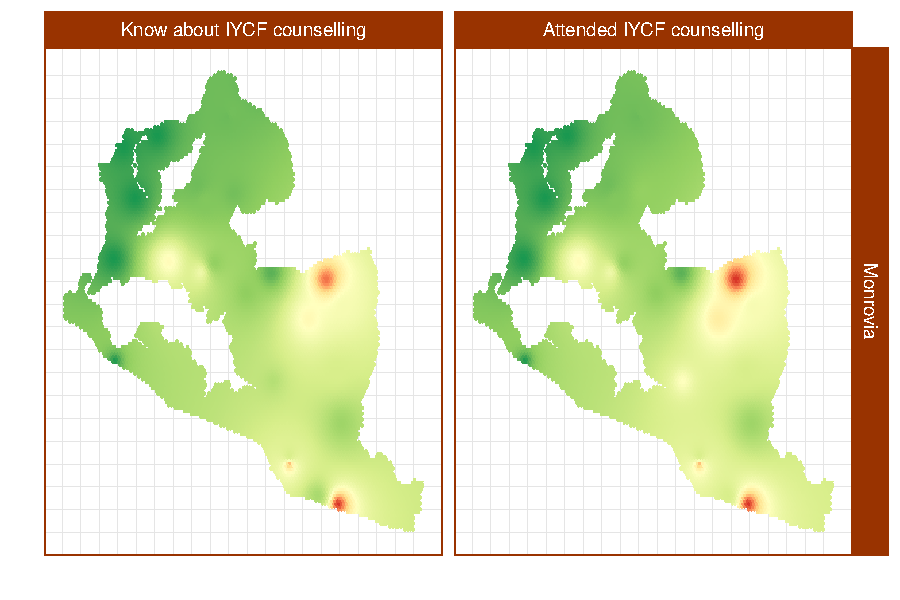
\includegraphics{liberiaCoverageReport_files/figure-latex/icfMap-1} 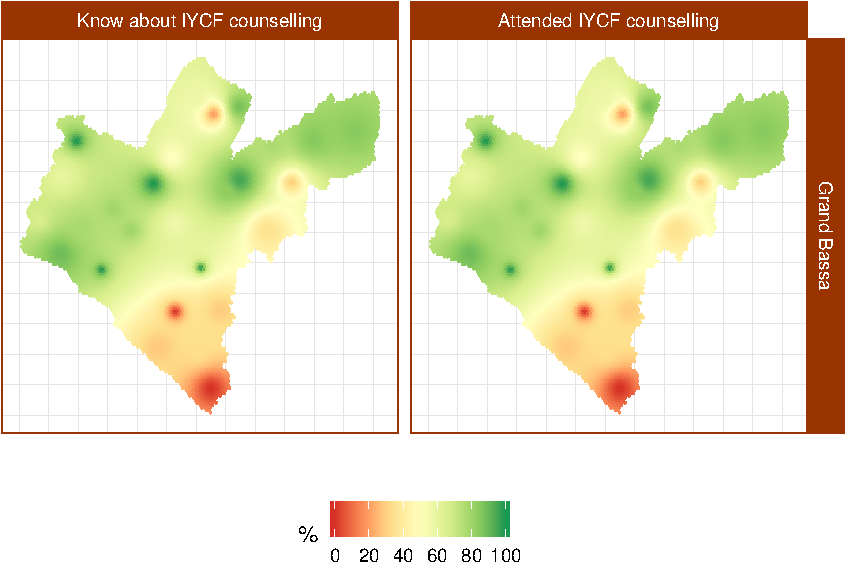
\includegraphics{liberiaCoverageReport_files/figure-latex/icfMap-2} 

}

\caption{Spatial Distribution of IYCF Counselling Coverage}\label{fig:icfMap}
\end{figure}

Of the few who do not attend IYCF counselling, their main reasons are
presented in \ref{fig:icf3a}.

\begin{figure}[H]

{\centering 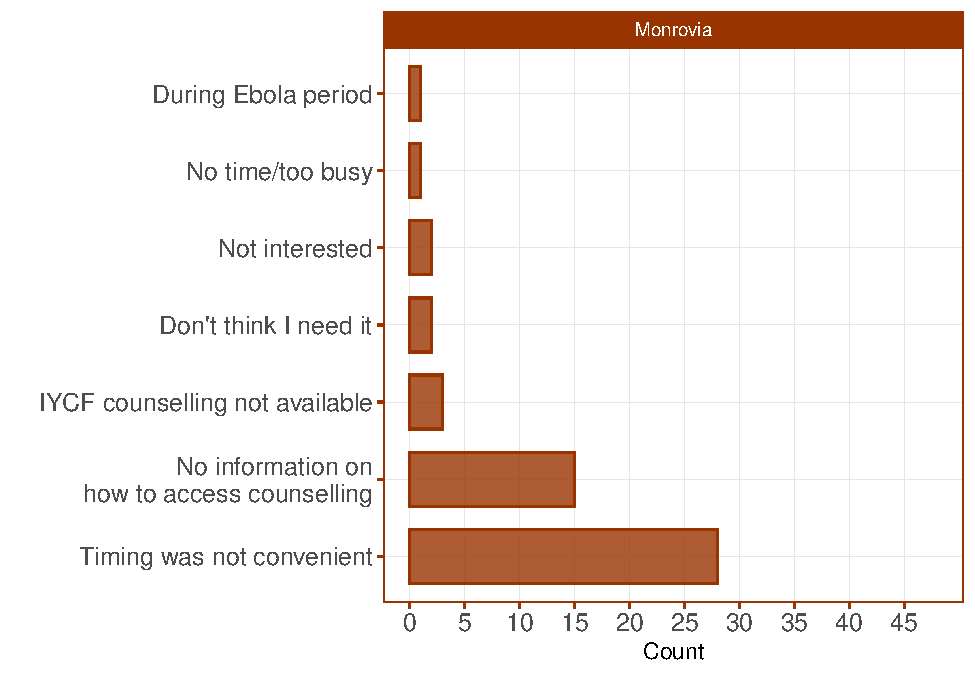
\includegraphics[width=8cm,height=6cm]{liberiaCoverageReport_files/figure-latex/icf3a-1} 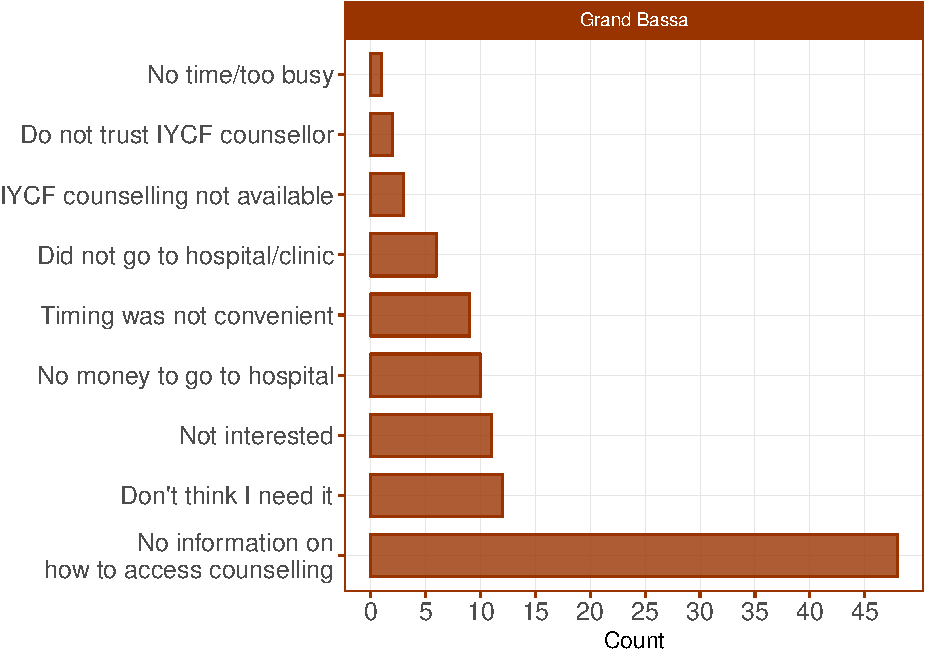
\includegraphics[width=8cm,height=6cm]{liberiaCoverageReport_files/figure-latex/icf3a-2} 

}

\caption{Reasons for not attending IYCF counselling}\label{fig:icf3a}
\end{figure}

\newpage

\hypertarget{micronutrient-powder-supplementation-coverage}{%
\subsection{Micronutrient Powder Supplementation
Coverage}\label{micronutrient-powder-supplementation-coverage}}

Figure \ref{fig:mnp1} and Table \ref{tab:mnp2} summarises the
hierarchical MNP supplementation coverage indicators. MNP
supplementation coverage is higher in Monrovia than in Grand Bassa but
both have low MNP supplementation coverage generally. Knowledge and
awareness of MNP is just under 18\% for Monrovia and just nearly 5\% for
Grand Bassa. Awareness of MNP supplementation is the main falter point
for achieving good MNP supplementation coverage.

\begin{figure}[H]

{\centering 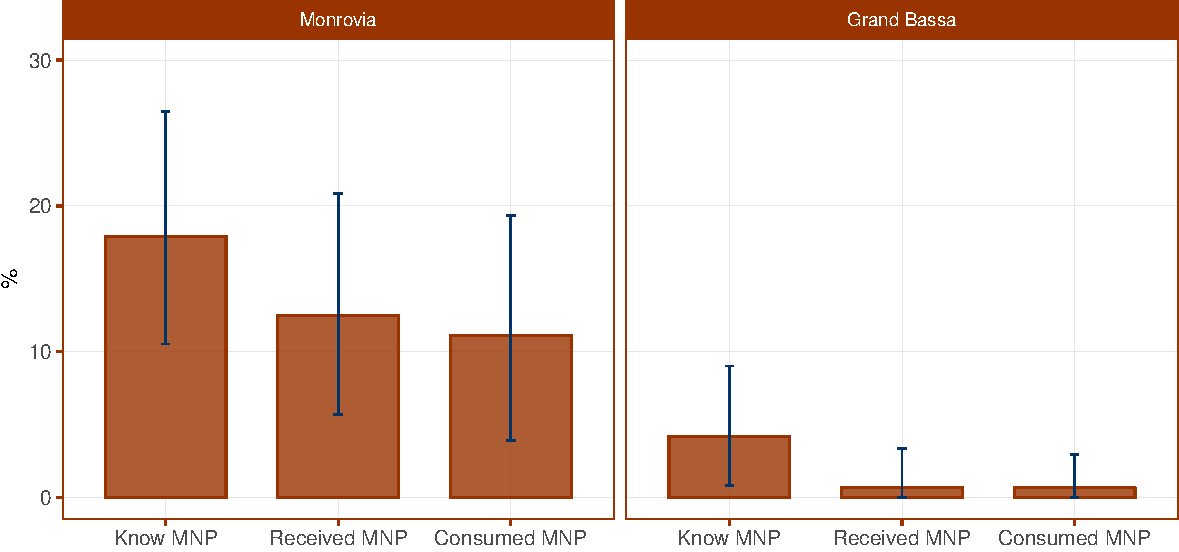
\includegraphics{liberiaCoverageReport_files/figure-latex/mnp1-1} 

}

\caption{Micronutrient Powder Supplementation Coverage}\label{fig:mnp1}
\end{figure}

\rowcolors{2}{gray!6}{white}\begin{table}[H]

\caption{\label{tab:mnp2}Micronutrient Powder Supplementation Coverage}
\centering
\fontsize{10}{12}\selectfont
\begin{tabular}[t]{lrrrrrr}
\hiderowcolors
\toprule
\multicolumn{1}{c}{\bfseries  } & \multicolumn{3}{c}{\bfseries Monrovia} & \multicolumn{3}{c}{\bfseries Grand Bassa} \\
\cmidrule(l{2pt}r{2pt}){2-4} \cmidrule(l{2pt}r{2pt}){5-7}
\textbf{Indicator} & \textbf{Estimate} & \textbf{95\% LCL} & \textbf{95\% UCL} & \textbf{Estimate} & \textbf{95\% LCL} & \textbf{95\% UCL}\\
\midrule
\showrowcolors
Know MNP & 17.93 & 10.54 & 26.50 & 4.23 & 0.82 & 9.03\\
Received MNP & 12.50 & 5.70 & 20.84 & 0.71 & 0.00 & 3.36\\
Consumed MNP & 11.11 & 3.92 & 19.37 & 0.70 & 0.00 & 2.97\\
\bottomrule
\end{tabular}
\end{table}\rowcolors{2}{white}{white}

Spatial distribution of MNP supplementation coverage is across the board
low in majority of the areas of Monrovia and Grand Bassa except for
small pockets of high coverage as shown in Figure @ref(\citet{mnpMap}).

\begin{figure}[H]

{\centering 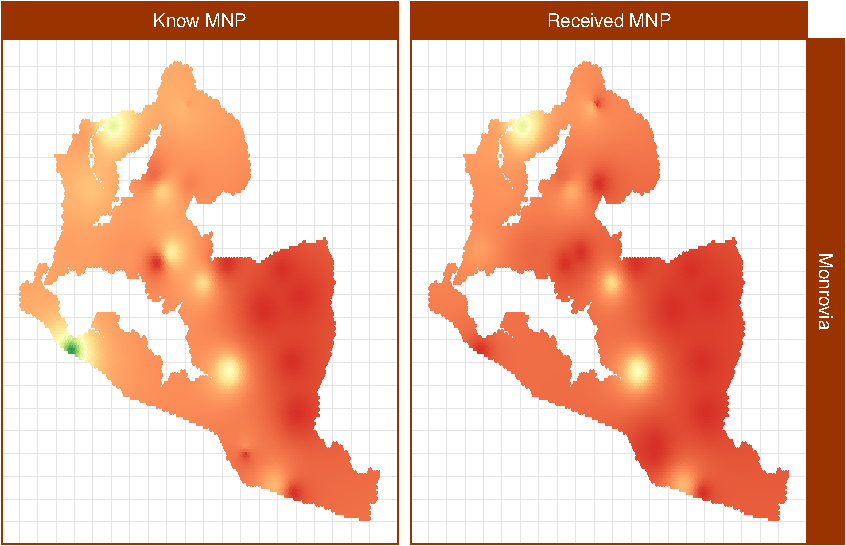
\includegraphics{liberiaCoverageReport_files/figure-latex/mnpMap-1} 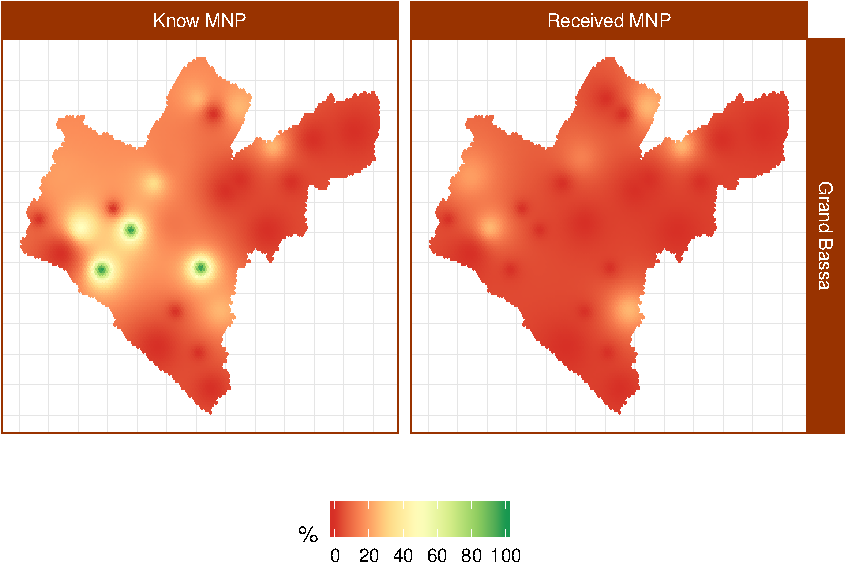
\includegraphics{liberiaCoverageReport_files/figure-latex/mnpMap-2} 

}

\caption{Spatial Distribution of MNP Supplementation Coverage}\label{fig:mnpMap}
\end{figure}

The main reasons for not receiving MNP supplements are presented in
Figure \ref{mnp3}. Lack of information on MNP supplementation is the
main reason for non-coverage consistent with MNP supplementation
coverage indicator results.

\begin{figure}[H]

{\centering 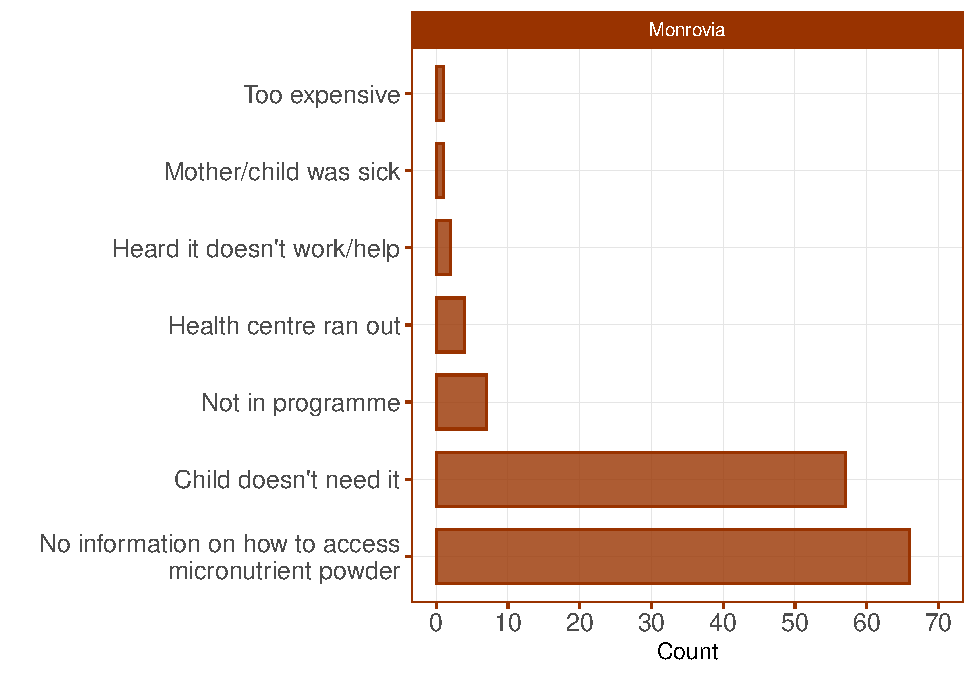
\includegraphics[width=8cm,height=6cm]{liberiaCoverageReport_files/figure-latex/mnp3a-1} 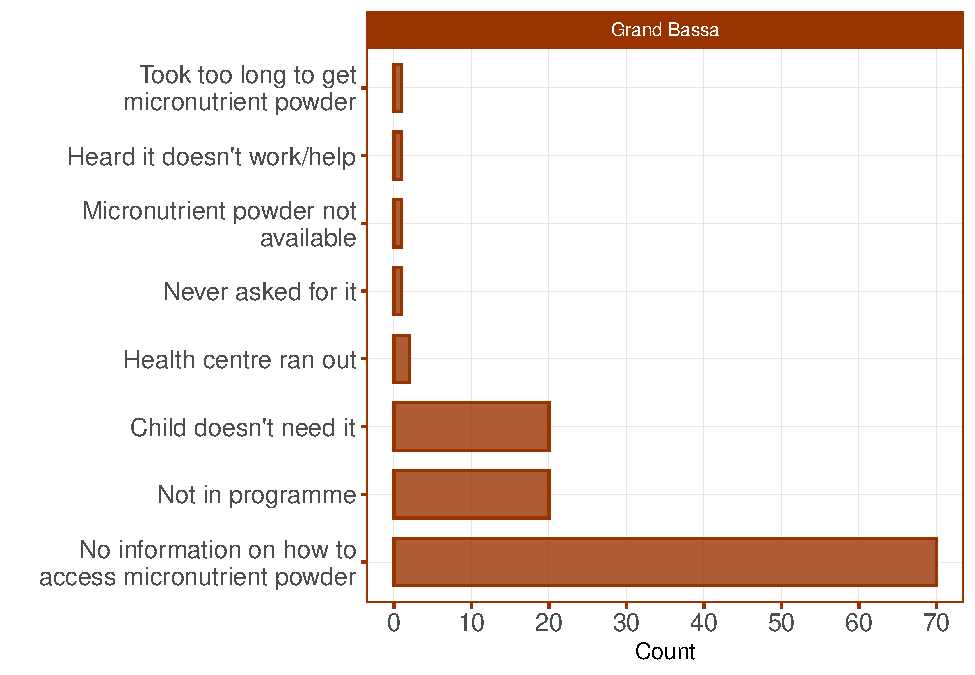
\includegraphics[width=8cm,height=6cm]{liberiaCoverageReport_files/figure-latex/mnp3a-2} 

}

\caption{Reasons for not receiving micronutrient powder}\label{fig:mnp3a}
\end{figure}

\newpage

\hypertarget{vitamin-a-supplementation-coverage}{%
\subsection{Vitamin A Supplementation
Coverage}\label{vitamin-a-supplementation-coverage}}

Vitamin A supplementation coverage is shown in Figure \ref{fig:vit1} and
Table \ref{tab:vit2}. There were 82\% and 85\% of children 6-59 months
in Monrovia and Grand Bassa respectively who received vitamin A
supplementation in the past 6 months. Provision of adequate dosage of
vitamin A supplementation is slightly lower at 65\% and 68\% in Monrovia
and Grand Bassa respectively. This is the potential falter point in
vitamin A supplementation for both programme areas.

\begin{figure}[H]

{\centering 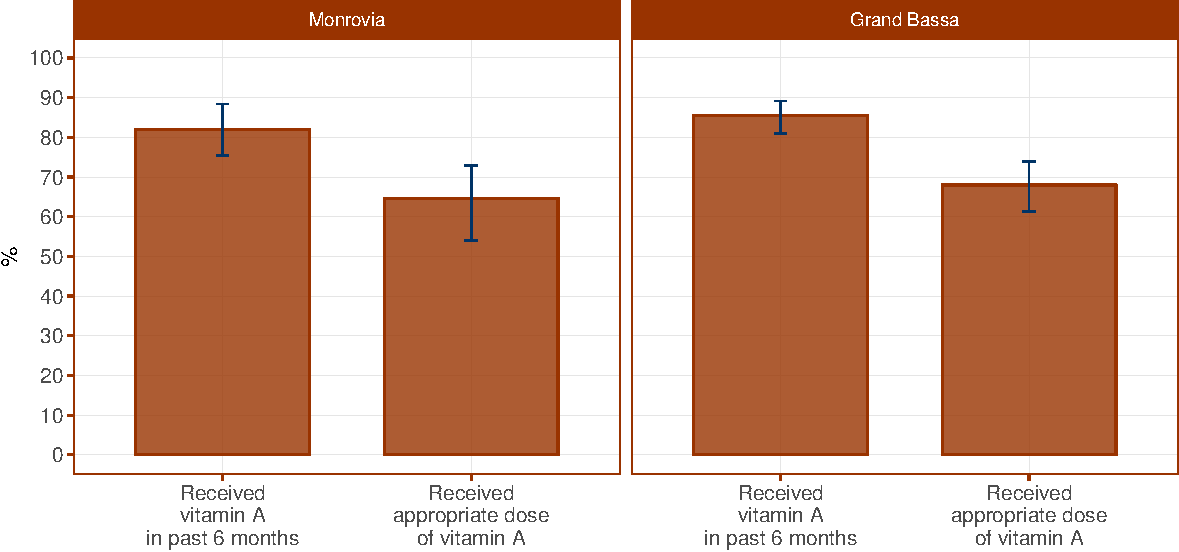
\includegraphics{liberiaCoverageReport_files/figure-latex/vit1-1} 

}

\caption{Vitamin A Supplementation Coverage}\label{fig:vit1}
\end{figure}

\rowcolors{2}{gray!6}{white}\begin{table}[H]

\caption{\label{tab:vit2}Vitamin A Supplementation Coverage}
\centering
\resizebox{\linewidth}{!}{
\fontsize{10}{12}\selectfont
\begin{tabular}[t]{lrrrrrr}
\hiderowcolors
\toprule
\multicolumn{1}{c}{\bfseries  } & \multicolumn{3}{c}{\bfseries Monrovia} & \multicolumn{3}{c}{\bfseries Grand Bassa} \\
\cmidrule(l{2pt}r{2pt}){2-4} \cmidrule(l{2pt}r{2pt}){5-7}
\textbf{Indicator} & \textbf{Estimate} & \textbf{95\% LCL} & \textbf{95\% UCL} & \textbf{Estimate} & \textbf{95\% LCL} & \textbf{95\% UCL}\\
\midrule
\showrowcolors
Received vitamin A in past 6 months & 82.06 & 75.44 & 88.41 & 85.46 & 80.95 & 89.19\\
Received appropriate dose of vitamin A & 64.65 & 53.94 & 72.87 & 67.98 & 61.32 & 73.87\\
\bottomrule
\end{tabular}}
\end{table}\rowcolors{2}{white}{white}

Spatial distribution of vitamin A supplementation is shown in Figure
\ref{fig:vitMap}. The south and eastern areas of Monrovia and the
southern area of Grand Bassa have the lowest vitamin A supplementation
coverage.

\begin{figure}[H]

{\centering 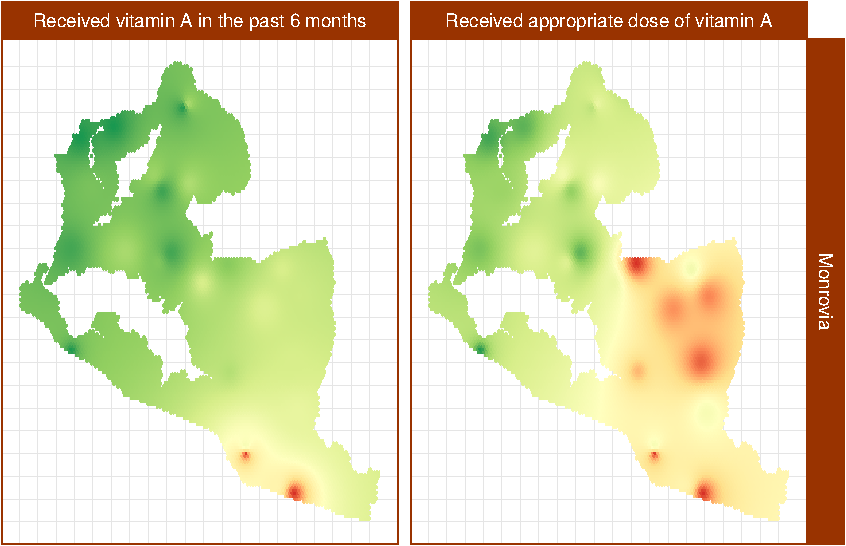
\includegraphics{liberiaCoverageReport_files/figure-latex/vitMap-1} 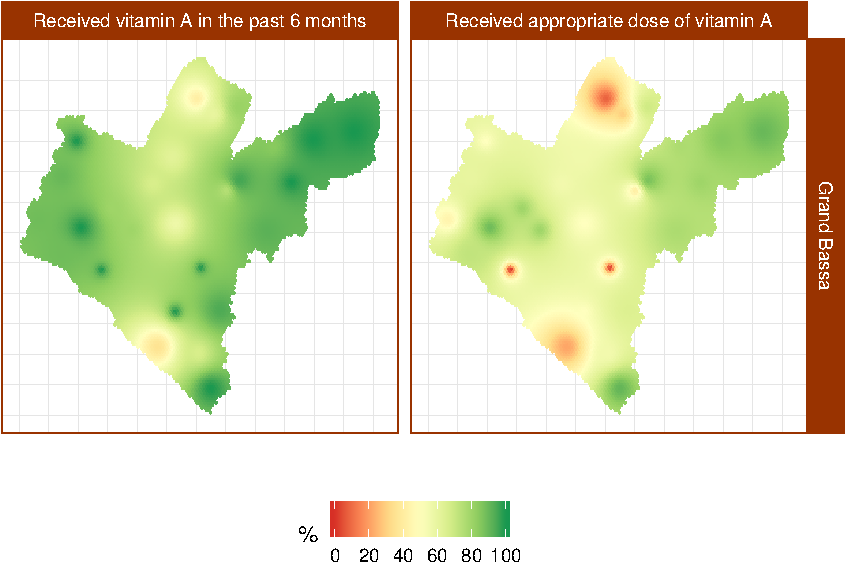
\includegraphics{liberiaCoverageReport_files/figure-latex/vitMap-2} 

}

\caption{Spatial Distribution of Vitamin A Coverage}\label{fig:vitMap}
\end{figure}

The main reasons for not receiving vitamin A are presented in Figure
\ref{fig:vit3}.

\begin{figure}[H]

{\centering 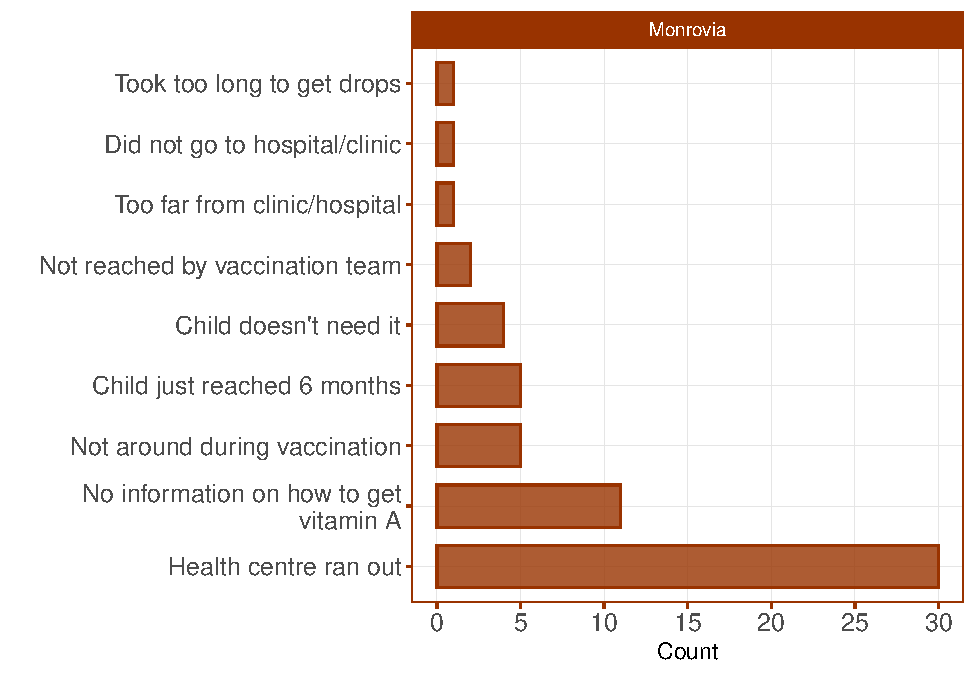
\includegraphics[width=8cm,height=6cm]{liberiaCoverageReport_files/figure-latex/vit3a-1} 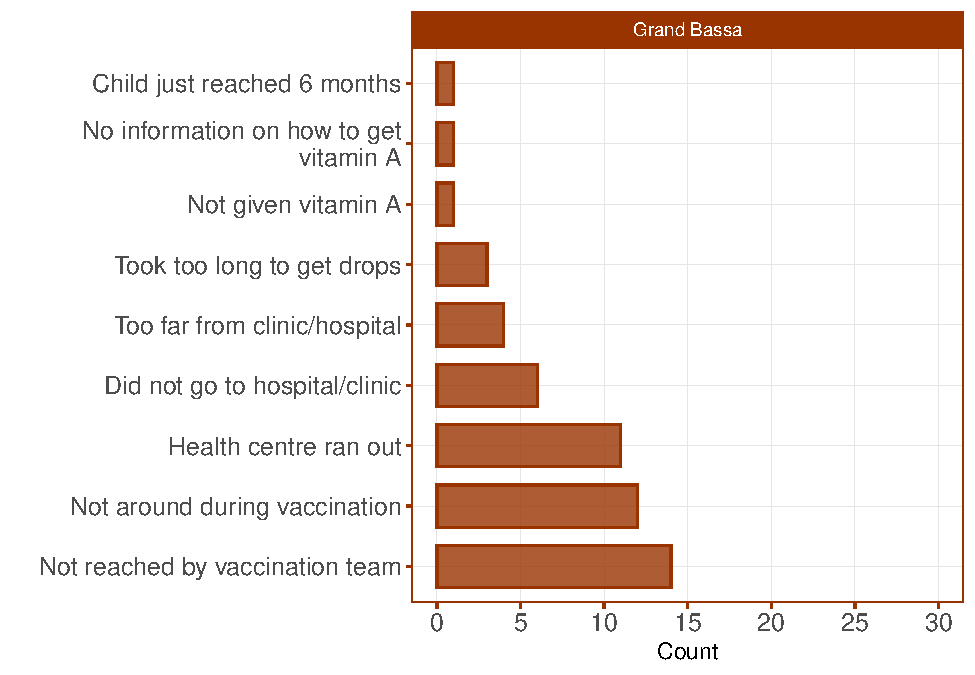
\includegraphics[width=8cm,height=6cm]{liberiaCoverageReport_files/figure-latex/vit3a-2} 

}

\caption{Reasons for not receiving vitamin A}\label{fig:vit3a}
\end{figure}

\newpage

\hypertarget{acute-undernutrition-prevalence}{%
\subsection{Acute undernutrition
prevalence}\label{acute-undernutrition-prevalence}}

Prevalence of acute undernutrition is presented in Figure \ref{fig:nut1}
and Table \ref{tab:nut2}. Acute undernutrition rates were highest in
Grand Bassa reaching up to 4\% GAM and close to 2\% GAM in Monrovia.
These estimates are relatively low but are the generally expected values
for these areas in Liberia.

\begin{figure}[H]

{\centering 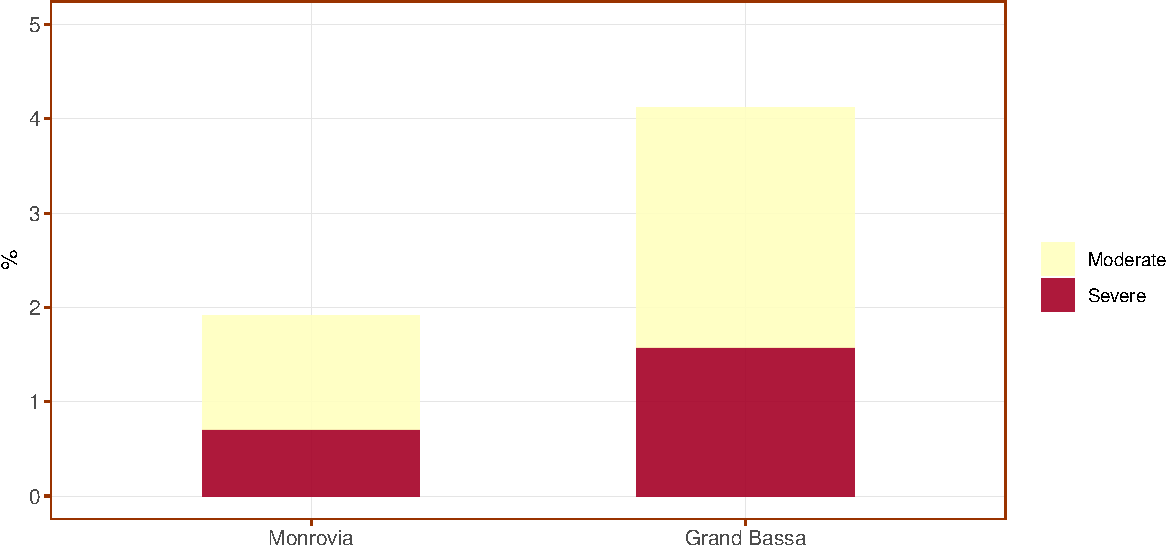
\includegraphics{liberiaCoverageReport_files/figure-latex/nut1-1} 

}

\caption{Acute Undernutrition Prevalence}\label{fig:nut1}
\end{figure}

\rowcolors{2}{gray!6}{white}\begin{table}[H]

\caption{\label{tab:nut2}Acute undernutrition prevalence}
\centering
\resizebox{\linewidth}{!}{
\fontsize{10}{12}\selectfont
\begin{tabular}[t]{lrrrrrr}
\hiderowcolors
\toprule
\multicolumn{1}{c}{\bfseries  } & \multicolumn{3}{c}{\bfseries Monrovia} & \multicolumn{3}{c}{\bfseries Grand Bassa} \\
\cmidrule(l{2pt}r{2pt}){2-4} \cmidrule(l{2pt}r{2pt}){5-7}
\textbf{Indicator} & \textbf{Estimate} & \textbf{95\% LCL} & \textbf{95\% UCL} & \textbf{Estimate} & \textbf{95\% LCL} & \textbf{95\% UCL}\\
\midrule
\showrowcolors
Global acute malnutrition & 1.91 & 1.29 & 2.73 & 4.19 & 3.45 & 5.04\\
Moderate acute malnutrition & 1.21 & 0.78 & 1.72 & 2.54 & 2.02 & 3.22\\
Severe acute malnutrition & 0.71 & 0.32 & 1.14 & 1.58 & 1.07 & 2.14\\
\bottomrule
\end{tabular}}
\end{table}\rowcolors{2}{white}{white}

Acute undernutrition is generally low all over Monrovia and Grand Bassa
with small pockets of high prevalence as shown in Figure
\ref{fig:nutMap}.

\begin{figure}[H]

{\centering 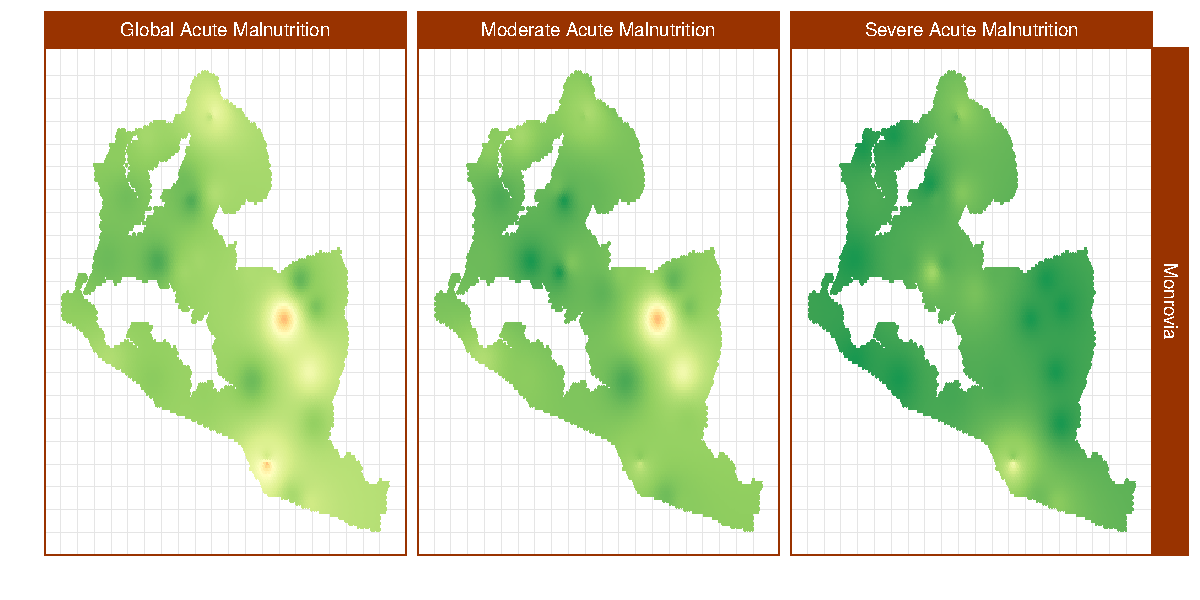
\includegraphics{liberiaCoverageReport_files/figure-latex/nutMap-1} 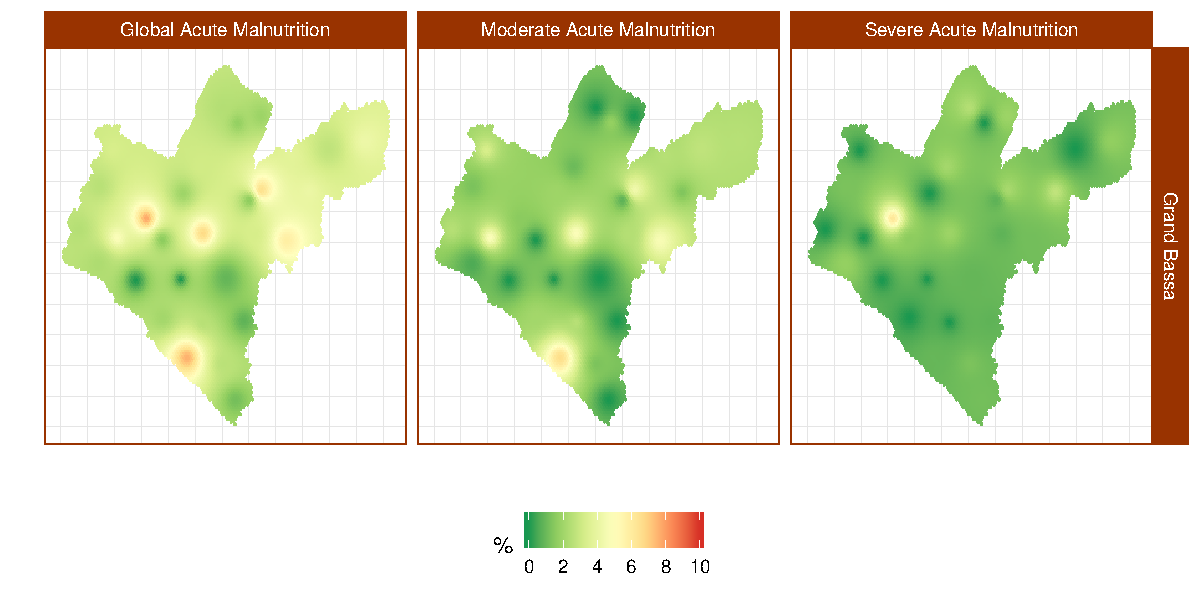
\includegraphics{liberiaCoverageReport_files/figure-latex/nutMap-2} 

}

\caption{Spatial Distribution of Acute Undernutrition Prevalence}\label{fig:nutMap}
\end{figure}

\newpage

\hypertarget{acute-undernutrition-screening-coverage}{%
\subsection{Acute undernutrition screening
coverage}\label{acute-undernutrition-screening-coverage}}

Screening coverage is very low for both Monrovia and Grand Bassa as
shown in Figure \ref{fig:screen1} and Table \ref{tab:screen2} and
spatial distribution is low across all areas of both programme areas as
shown in the maps in Figure \ref{fig:screenMap}.

\begin{figure}[H]

{\centering 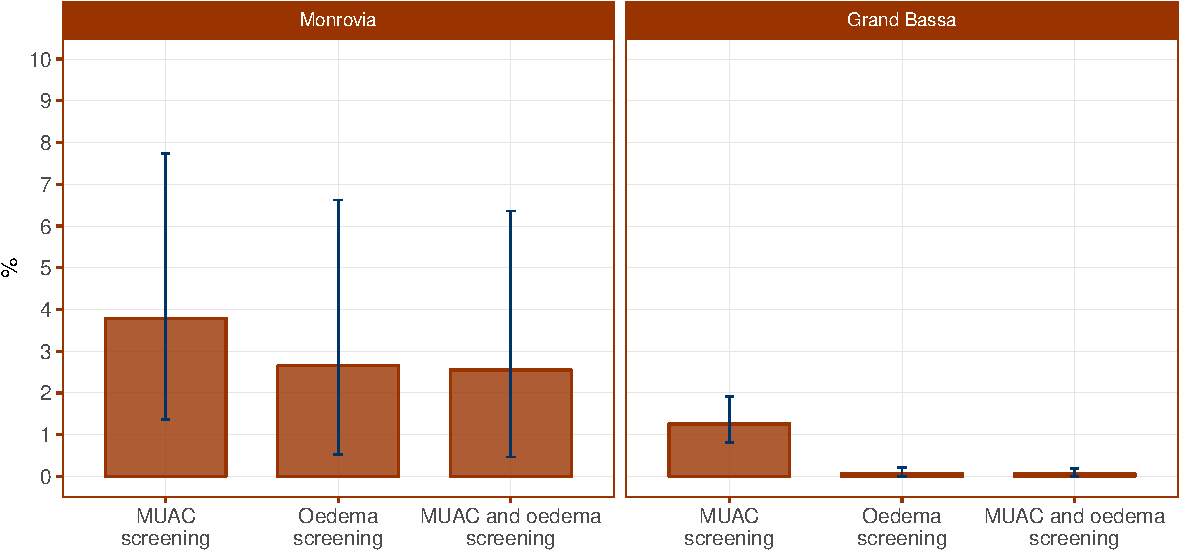
\includegraphics{liberiaCoverageReport_files/figure-latex/screen1-1} 

}

\caption{Acute Undernutrition Screening Coverage}\label{fig:screen1}
\end{figure}

\rowcolors{2}{gray!6}{white}\begin{table}[H]

\caption{\label{tab:screen2}Acute undernutrition screening coverage}
\centering
\resizebox{\linewidth}{!}{
\fontsize{10}{12}\selectfont
\begin{tabular}[t]{lrrrrrr}
\hiderowcolors
\toprule
\multicolumn{1}{c}{\bfseries  } & \multicolumn{3}{c}{\bfseries Monrovia} & \multicolumn{3}{c}{\bfseries Grand Bassa} \\
\cmidrule(l{2pt}r{2pt}){2-4} \cmidrule(l{2pt}r{2pt}){5-7}
\textbf{Indicator} & \textbf{Estimate} & \textbf{95\% LCL} & \textbf{95\% UCL} & \textbf{Estimate} & \textbf{95\% LCL} & \textbf{95\% UCL}\\
\midrule
\showrowcolors
MUAC Screening & 3.79 & 1.37 & 7.73 & 1.26 & 0.81 & 1.92\\
Oedema Screening & 2.65 & 0.52 & 6.63 & 0.07 & 0.00 & 0.21\\
MUAC and Oedema Screening & 2.55 & 0.46 & 6.36 & 0.06 & 0.00 & 0.19\\
\bottomrule
\end{tabular}}
\end{table}\rowcolors{2}{white}{white}

\begin{figure}[H]

{\centering 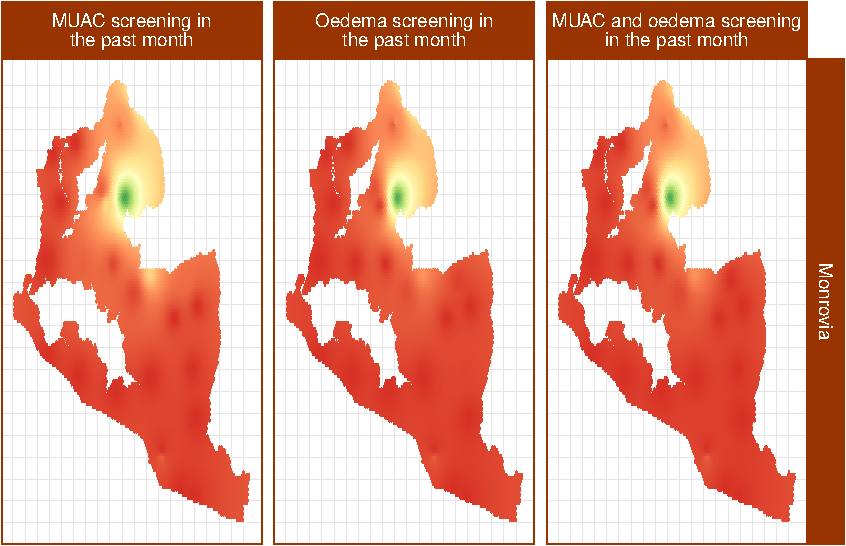
\includegraphics{liberiaCoverageReport_files/figure-latex/screenMap-1} 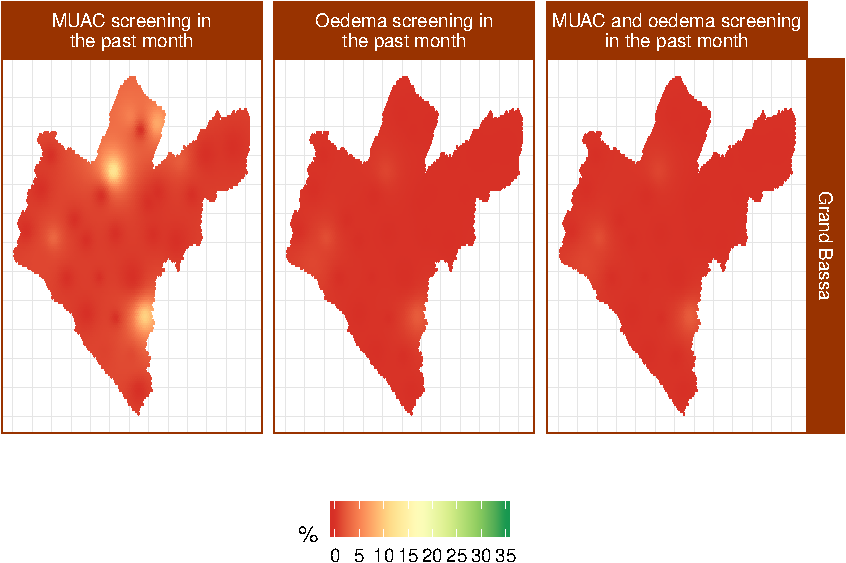
\includegraphics{liberiaCoverageReport_files/figure-latex/screenMap-2} 

}

\caption{Spatial Distribution of Acute Undernutrition Screening Coverage}\label{fig:screenMap}
\end{figure}

\newpage

\hypertarget{cmam-coverage-1}{%
\subsection{CMAM Coverage}\label{cmam-coverage-1}}

Case-finding effectiveness in both Monrovia and Grand Bassa are low (see
Figure \ref{fig:cmam1} and Table \ref{tab:cmam2}) with Monrovia having a
higher rate at about 31\% compared to 6\% in Grand Bassa. Treatment
coverage is at 55\% in Monrovia which is an improvement from previous
coverage estimates for the area but Grand Bassa only managed to get 18\%
treatment coverage.

\begin{figure}[H]

{\centering 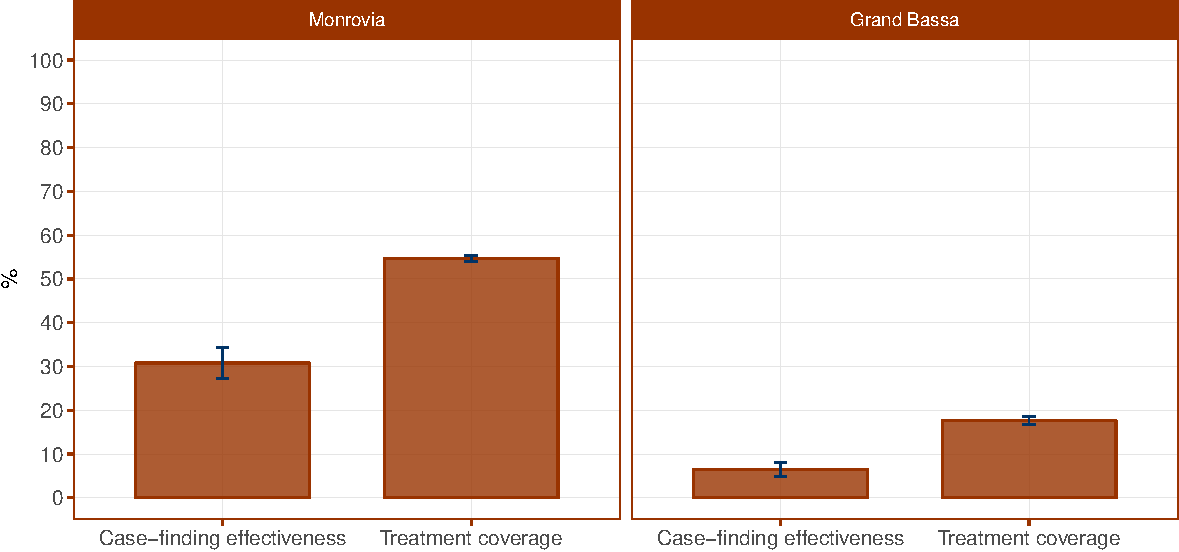
\includegraphics{liberiaCoverageReport_files/figure-latex/cmam1-1} 

}

\caption{CMAM Coverage}\label{fig:cmam1}
\end{figure}

\rowcolors{2}{gray!6}{white}\begin{table}[H]

\caption{\label{tab:cmam2}CMAM coverage}
\centering
\resizebox{\linewidth}{!}{
\fontsize{10}{12}\selectfont
\begin{tabular}[t]{lrrrrrr}
\hiderowcolors
\toprule
\multicolumn{1}{c}{\bfseries  } & \multicolumn{3}{c}{\bfseries Monrovia} & \multicolumn{3}{c}{\bfseries Grand Bassa} \\
\cmidrule(l{2pt}r{2pt}){2-4} \cmidrule(l{2pt}r{2pt}){5-7}
\textbf{Indicator} & \textbf{Estimate} & \textbf{95\% LCL} & \textbf{95\% UCL} & \textbf{Estimate} & \textbf{95\% LCL} & \textbf{95\% UCL}\\
\midrule
\showrowcolors
Case-finding effectiveness & 30.77 & 27.29 & 34.25 & 6.45 & 4.90 & 8.00\\
Treatment coverage & 54.68 & 53.97 & 55.38 & 17.65 & 16.77 & 18.53\\
\bottomrule
\end{tabular}}
\end{table}\rowcolors{2}{white}{white}

The spatial distribution of CMAM coverage (see Figure \ref{fig:cmamMap})
shows high levels of coverage throughout most of Monrovia but with
significant areas of low coverage in the western and southeastern
sections. For Grand Bassa, coverage is low throughout most of Grand
Bassa but with pockets of high coverage in the western area of the
county.

\begin{figure}[H]

{\centering 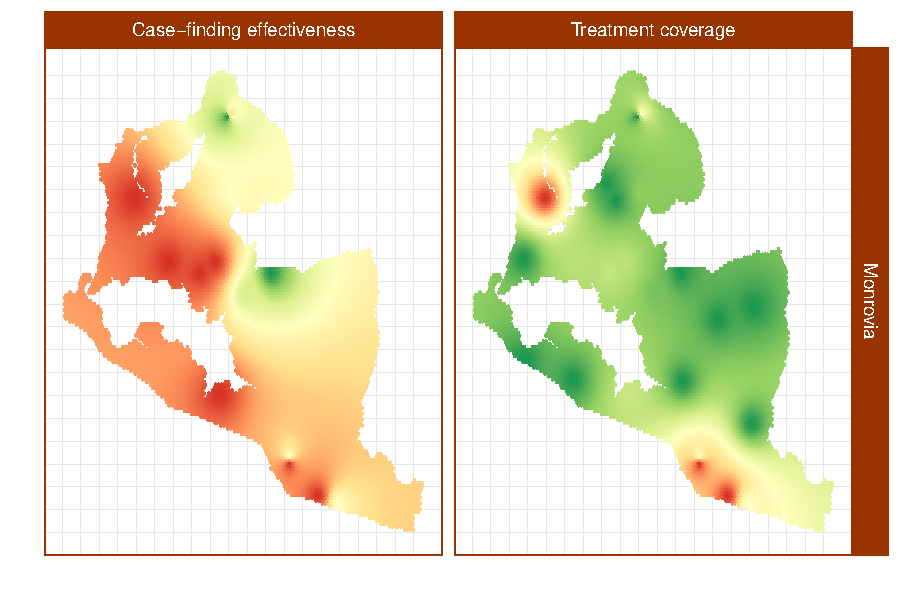
\includegraphics{liberiaCoverageReport_files/figure-latex/cmamMap-1} 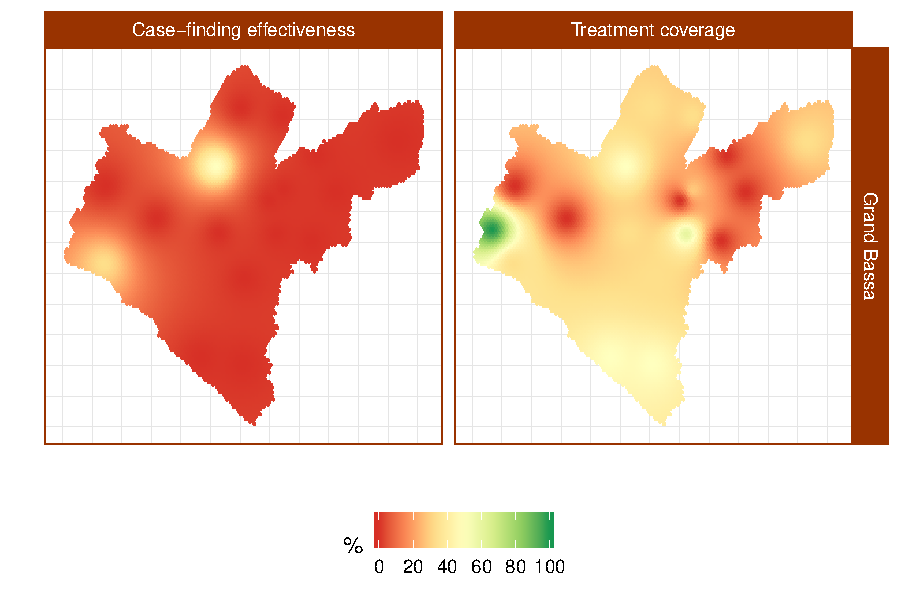
\includegraphics{liberiaCoverageReport_files/figure-latex/cmamMap-2} 

}

\caption{Spatial Distribution of CMAM Coverage}\label{fig:cmamMap}
\end{figure}

For SAM cases not covered by the programme, Figure \ref{fig:cmam3}
summarises the reasons for non-coverage.

\begin{figure}[H]

{\centering 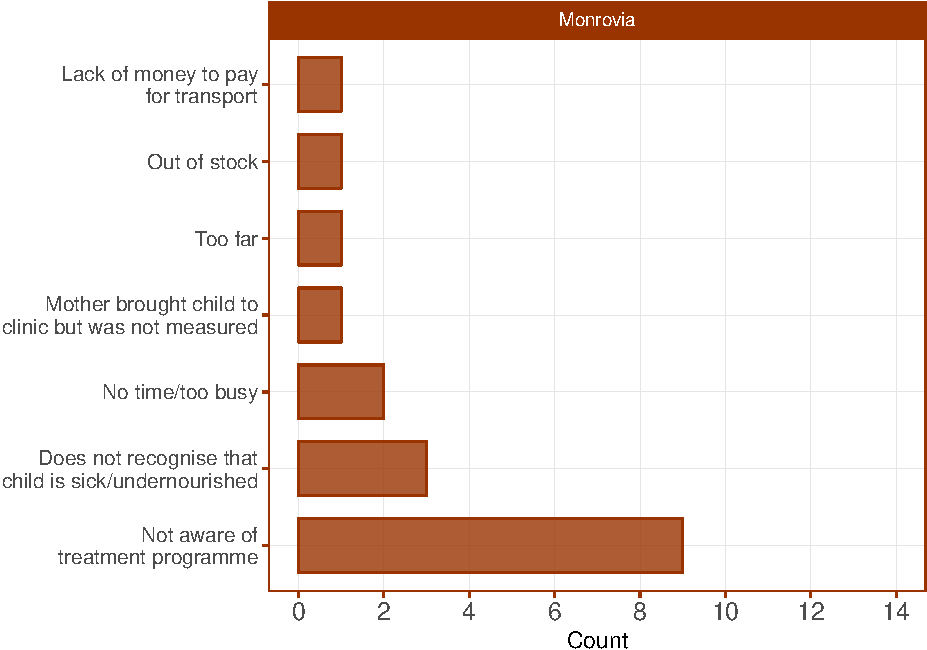
\includegraphics[width=8cm,height=16cm]{liberiaCoverageReport_files/figure-latex/cmam3-1} 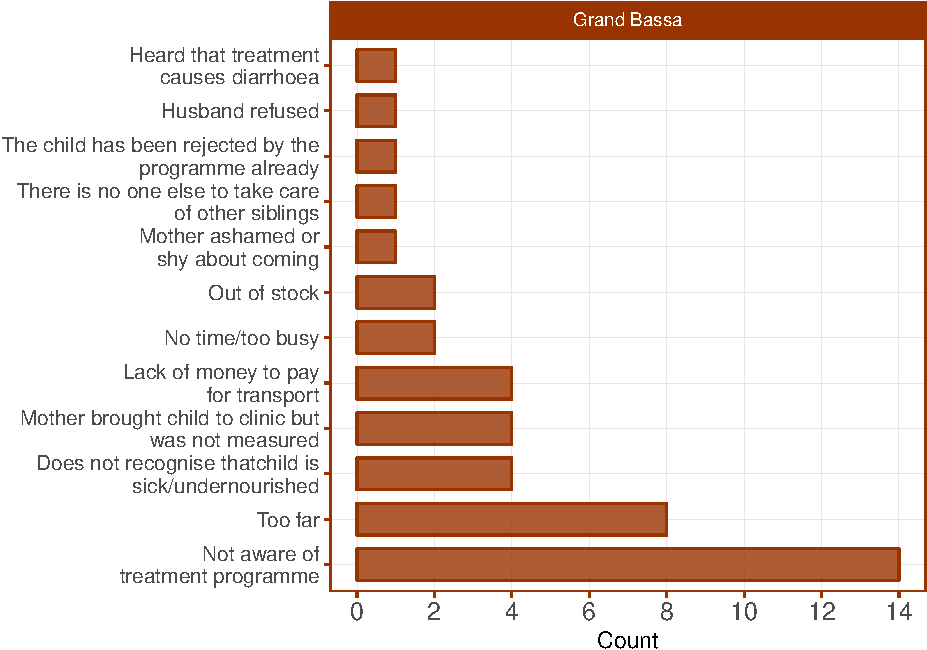
\includegraphics[width=8cm,height=16cm]{liberiaCoverageReport_files/figure-latex/cmam3-2} 

}

\caption{Reasons for not being in CMAM programme}\label{fig:cmam3}
\end{figure}

\hypertarget{discussion}{%
\section{Discussion}\label{discussion}}

The results of the first midterm coverage assessment of direct nutrition
interventions in Liberia specifically in Monrovia and Grand Bassa
indicate various levels of disparity in coverage based on how long the
direct nutrition intervention has been in place and in location both
between the programme areas assessed and within the programme areas
assessed.

Long-standing programmes such as IFA, IYCF counselling and vitamin A
supplementation have performed fairly well in terms of coverage. The
majority of women and children targeted by these programmes are
knowledgeable of the programme and are beneficiaries of the programme.
Years of implementation complemented by the level of support and
investment by the government and its partners seem to have paid
dividends in allowing for these programmes to reach almost all of their
targeted beneficiaries. However, there is still much room for
improvement and the current coverage levels can still be improved and
increased.

For IFA supplementation, the programme has been able to reach most
mothers and has been successful in getting them to take IFA supplements.
However, the key challenge for the programme now is to keep mothers
taking the tablets for the recommended period of time (at least 90
days). Currently, most of the mothers stop before 2 months of
supplementation which is quite soon. Whilst the survey does not collect
data on mother's reasons for stopping IFA tablet consumption, the most
common reason for not continuing at this early stage is because of side
effects caused by the IFA tablets. Given that contact with health care
services during pregnancy is high, it would be good to review existing
guidance provided through ANC regarding the intake of IFA and to see
whether relevant and appropriate information on correct usage of IFA and
its known side effects and ways by which to minimise them are included
and/or emphasised.

For IYCF counselling, the survey only assessed knowledge and attendance
of IYCF counselling. The natural next level in the coverage hierarchy is
whether mothers practice what they have been taught. The most
straightforward way of doing so would be assessing IYCF practices as
these are the key behaviours that are targeted by the counselling. If
this was to be considered, however, UNICEF and its partners would have
to take into account the fact that current standard IYCF indicators can
only be assessed through big sample surveys such as DHS and MICS. Yet
these surveys would most likely not provide the same level of detail and
information as current assessment. However, there are small sample
alternatives to the standard IYCF indicators such as the Infant and
Child Feeding Index (ICFI) indicator set \citep{Guevarra:2016uw}.

For vitamin A supplementation, the current figures are relatively lower
than the expected indirect coverage estimates produced by government. It
would be important to see what the potential reasons for this disparity
are and to ensure that vaccination campaigns, to which vitamin A
supplementation is generally attached, does not neglect vitamin A
supplementation as it seems access to vaccination is the key reason for
non-coverage.

Programmes such as MNP and CMAM, on the other hand, show how new and
recently scaled-up programmes are still in the process of achieving the
highest levels of coverage possible. MNP supplementation which is the
newest programme of those assessed is understandably still struggling
with coverage at its early stages of implementation. Knowledge of the
programme is the key falter point which is typical of a programme at
this stage of its evolution. The programme is mainly anchored to the
health centre and therefore knowledge and access to it is primarily
influenced by mothers' behaviours and attitudes towards seeking care and
treatment at the health facility. Given that MNP is aimed at children
who are otherwise healthy (not acute malnourished), the current MNP
coverage estimates indicate that health-seeking behaviour leading to a
visit to a health facility is mainly influenced by whether their
children are sick rather than as a way to seek information or
participate in promotive and preventive services such as MNP
supplementation. Other factors include physical access to health
centres. A more community-based approach to MNP supplementation that is
integrated with other community-based programmes such as vaccinations
and CMAM should be considered as a potential delivery mechanism.

Finally, for CMAM which is not entirely new but still in its early
stages of scale-up, the current coverage estimate shows potential
disparity between Monrovia and Grand Bassa in terms of the level and
intensity of the community aspects of the programme. Screening and
case-finding in Monrovia is better than in Grand Bassa and this can
partly explain the difference in treatment coverage between the two
areas. However, screening and case-finding is still an issue for both
areas hence their potential for achieving better coverage than is
currently being achieved. Monrovia, despite having a relatively lower
level of acute undernutrition, seem to have a higher intensity of
support and focus with regard to CMAM implementation as compared to
Grand Bassa where there are only 7 health facilities currently providing
CMAM services. It would be important to revisit how the programme has
been rolled out and is currently being scaled up in Grand Bassa and to
allocate CMAM services accordingly to the level of need in the county.
The spatial distribution maps of acute undernutrition in relation to the
CMAM coverage level maps can guide the prioritisation of which areas
will require health facilities providing CMAM services.

Lessons learned from the years of implementation of the IFA and vitamin
A programmes can be useful in improving coverage of MNP and CMAM
particularly with potential integration of these services into a unified
and coherent child health and nutrition programme in Liberia.

\renewcommand\refname{References}
\bibliography{bibliography.bib}


\end{document}
